\begin{center}
	\textbf{ÔN TẬP CHƯƠNG 2 HH 12}	
\end{center}
\Opensolutionfile{ans}[ans/ansCD2H2-3OTC]

\begin{ex}%[2H2B1-1]%[Thành Đức Trung]%Câu 1.
	Cho khối nón có chiều cao bằng $24$ cm, độ dài đường sinh bằng $26$ cm. Tính thể tích $V$ của khối nón tương ứng. 
	\choice
	{$V=800\pi$ cm$^3$}
	{$V=1600\pi$ cm$^3$}
	{$V=\dfrac{1600\pi}{3}$ cm$^3$}
	{\True $V=\dfrac{800\pi}{3}$ cm$^3$}
	\loigiai{
		Bán kính đáy của hình nón $R=\sqrt{\ell^2-h^2}=10$ cm.\\
		Vậy thể tích khối nón tương ứng là $V=\dfrac{1}{3}\pi R^2\cdot h=\dfrac{1}{3}\pi\cdot 100\cdot 24=\dfrac{800\pi}{3}$.}
\end{ex}

\begin{ex}%[2H2Y1-1]%[Thành Đức Trung]%Câu 2.
	Cho hình nón tròn xoay có bán kính đường tròn đáy $r$, chiều cao $h$ và đường sinh $\ell$. Kết luận nào sau đây \textbf{sai}?
	\choice
	{$V=\dfrac{1}{3}\pi r^2h$}
	{$S_{tp}=\pi r\ell+\pi r^2$}
	{\True $h^2=r^2+\ell^2$}
	{$S_{xq}=\pi r\ell$}
	\loigiai{
		\immini{
			Ta có tam giác $SOB$ vuông tại $O$ nên \[h^2+r^2=\ell^2\Rightarrow h^2=\ell^2-r^2.\]
		}{
			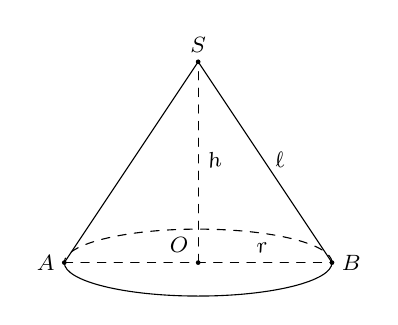
\begin{tikzpicture}[scale=0.85, font=\footnotesize, line join=round, line cap=round, >=stealth]
			\draw[dashed] (2,0) arc [start angle=0,end angle=180, x radius=2,y radius=1/2];
			\draw (-2,0) arc [ start angle=180, end angle=360, x radius=2,y radius=1/2];
			\draw[dashed] (-2,0)--(2,0) node[pos=0.75,above,rotate=10]{$ r $};
			\draw [dashed] (0,0)--(0,3) node[pos=0.5,right,rotate=10]{$ h $};
			\draw (-2,0) node[left]{$A$}--(0,3);
			\draw (0,3) node[above]{$S$}--(2,0) node[pos=0.5,right,rotate=10]{$\ell $};
			\fill (0,0) circle(1pt) (-2,0) circle(1pt) (2,0) circle(1pt) (0,3) circle(1pt);
			\draw (2,0) node[right]{$B$} (0,0) node[above left]{$O$};
			\end{tikzpicture}
		}
	}
\end{ex}

\begin{ex}%[2H2B1-1]%[Thành Đức Trung]%Câu 3.
	Cho tam giác $ABC$ vuông tại $A$. Khi quay tam giác đó quanh cạnh góc vuông $AB$, đường gấp khúc $BCA$ tạo thành hình tròn xoay nào trong bốn hình sau đây?
	\choice
	{\True Hình nón}
	{Hình trụ}
	{Hình cầu}
	{Hình tròn}
	\loigiai{
		Khi quay tam giác đó quanh cạnh góc vuông $AB$, đường gấp khúc $BCA$ tạo thành hình tròn xoay là hình nón.}
\end{ex}

\begin{ex}%[2H2Y1-1]%[Thành Đức Trung]%Câu 4.
	Cho hình nón có độ dài đường sinh $\ell=4a$ và bán kính đáy $r=a\sqrt{3}$. Diện tích xung quanh của hình nón bằng.
	\choice
	{$12\pi a^2\sqrt{3}$}
	{$\dfrac{4\pi a^2\sqrt{3}}{3}$}
	{$8\pi a^2\sqrt{3}$}
	{\True $4\pi a^2\sqrt{3}$}
	\loigiai{
		Ta có $S_{\text{xq}}=\pi r\ell =\pi\cdot a\sqrt{3}\cdot 4a =4\pi a^2\sqrt{3}$.}
\end{ex}

\begin{ex}%[2H2Y1-1]%[Thành Đức Trung]%Câu 5.
	Cho khối nón có bán kính đáy $r=\sqrt{3}$ và chiều cao $h=4$. Tính thể tích $V$ của khối nón đã cho. 
	\choice
	{$V=\dfrac{16\pi\sqrt{3}}{3}$}
	{\True $V=4\pi$}
	{$V=16\pi\sqrt{3}$}
	{$V=12\pi$}
	\loigiai{
		\immini{
			Thể tích khối nón $V=\dfrac{1}{3}\pi r^2h=4\pi$.
		}{
			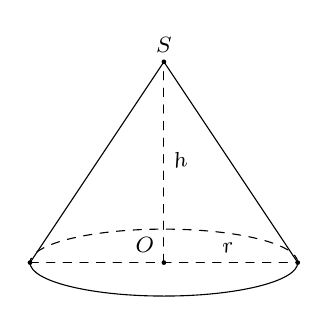
\begin{tikzpicture}[scale=0.85, font=\footnotesize, line join=round, line cap=round, >=stealth]
			\draw[dashed] (2,0) arc [start angle=0,end angle=180, x radius=2,y radius=1/2];
			\draw (-2,0) arc [ start angle=180, end angle=360, x radius=2,y radius=1/2];
			\draw[dashed] (-2,0)--(2,0) node[pos=0.75,above,rotate=10]{$ r $};
			\draw [dashed] (0,0)--(0,3) node[pos=0.5,right,rotate=10]{$ h $};
			\draw (-2,0)--(0,3);
			\draw (0,3) node[above]{$S$}--(2,0);
			\fill (0,0) circle(1pt) (-2,0) circle(1pt) (2,0) circle(1pt) (0,3) circle(1pt);
			\draw (0,0) node[above left]{$O$};
			\end{tikzpicture}
		}	
	}
\end{ex}

\begin{ex}%[2H2Y1-2]%[Thành Đức Trung]%Câu 6.
	Cho hình trụ có chiều cao bằng $2a$, bán kính đáy bằng $a$. Tính diện tích xung quanh của hình trụ. 
	\choice
	{$\pi a^2$}
	{$2a^2$}
	{$2\pi a^2$}
	{\True $4\pi a^2$}
	\loigiai{
		Diện tích xung quanh $S=2\pi R\cdot h=2\pi\cdot a\cdot 2a=4\pi a^2$.}
\end{ex}

\begin{ex}%[2H2Y1-2]%[Thành Đức Trung]%Câu 7.
	Một hình trụ có bán kính đáy bằng $r$ và có thiết diện qua trục là một hình vuông. Khi đó diện tích toàn phần của hình trụ đó là
	\choice
	{\True $6\pi r^2$}
	{$2\pi r^2$}
	{$8\pi r^2$}
	{$4\pi r^2$}
	\loigiai{
		\begin{center}
			\begin{tikzpicture}[scale=0.7, font=\footnotesize, line join=round, line cap=round, >=stealth]
			\tikzset{label style/.style={font=\footnotesize}}
			\tkzDefPoints{0/0/O}
			\tkzDefShiftPoint[O](-120:2){A}
			\tkzDefShiftPoint[O](120:2){B}
			\tkzDefShiftPoint[O](60:2){C}
			\tkzDefShiftPoint[O](-60:2){D}
			\draw (D) arc (0:-180:2cm and 1cm);
			\draw[dashed] (D) arc (0:180:2cm and 1cm);
			\draw (C) arc (0:-360:2cm and 1cm);
			\coordinate (C') at ($2*(B)-(C)$);
			\coordinate (D') at ($2*(A)-(D)$);	
			\tkzDrawPoints[size=2](A,B,C,D)
			\tkzDrawSegments(B,C C',D' C,D)
			\tkzDrawSegments[dashed](A,B A,D)
			\tkzLabelSegment[right](C,D){$2r$}
			\tkzLabelSegment[left](A,B){$h$}
			\tkzLabelSegment[above](B,C){$r$}
			\tkzMarkRightAngle(B,A,D);
			\tkzMarkRightAngle(A,D,C);
			\end{tikzpicture}
		\end{center}
			Do thiết diện qua trục là hình vuông nên ta có $S_{\text{tp}}=S_{\text{xq}}+2S_{\text{đ}} =2\pi r\cdot 2r+2\pi r^2 =6\pi r^2$.
	}
\end{ex}

\begin{ex}%[2H2Y2-1]%[Thành Đức Trung]%Câu 8.
	Công thức tính diện tích mặt cầu bán kính $R$ là
	\choice
	{$S=\pi R^2$}
	{$S=\dfrac{4}{3}\pi R^3$}
	{$S=\dfrac{3}{4}\pi R^2$}
	{\True $S=4\pi R^2$}
	\loigiai{
		Công thức tính diện tích mặt cầu bán kính $R$ là $S=4\pi R^2$.}
\end{ex}

\begin{ex}%[2H2Y2-1]%[Thành Đức Trung]%Câu 9.
	Một hình cầu có bán kính bằng $2$. Hỏi diện tích của mặt cầu bằng bao nhiêu?
	\choice
	{$4\pi$}
	{\True $16\pi$}
	{$8\pi$}
	{$\pi$}
	\loigiai{
		Diện tích mặt cầu $S=4\pi R^2 =16\pi$.}
\end{ex}

\begin{ex}%[2H2Y2-1]%[Thành Đức Trung]%Câu 10.
	Cho mặt cầu có diện tích bằng $\dfrac{8\pi a^2}{3}$. Bán kính mặt cầu bằng
	\choice
	{\True $\dfrac{a\sqrt{6}}{3}$}
	{$\dfrac{a\sqrt{3}}{3}$}
	{$\dfrac{a\sqrt{6}}{2}$}
	{$\dfrac{a\sqrt{2}}{3}$}
	\loigiai{
		Diện tích mặt cầu $S=4\pi R^2\Leftrightarrow 4\pi R^2=\dfrac{8\pi a^2}{3}\Leftrightarrow R=\dfrac{a\sqrt{6}}{3}$.}
\end{ex}

\begin{ex}%[2H2B1-2]%[Thành Đức Trung]%Câu 11.
	Cho tam giác $AOB$ vuông tại $O$, có $\widehat{OAB}=30^{\circ}$ và $AB=a$. Quay tam giác $AOB$ quanh trục $AO$ ta được một hình nón. Tính diện tích xung quanh $S_{\text{xq}}$ của hình nón đó. 
	\choice
	{\True $\dfrac{\pi a^2}{2}$}
	{$S_{\text{xq}}=\pi a^2$}
	{$S_{\text{xq}}=\dfrac{\pi a^2}{4}$}
	{$S_{\text{xq}}=2\pi a^2$}
	\loigiai{
		\immini{
			$S_{\text{xq}}=\pi Rl$ trong đó $R=OB$, $l=AB$.\\
			Trong tam giác vuông $OAB$ ta có $OB=AB\cdot\sin 30^{\circ}$ hay $R=\dfrac{AB}{2}=\dfrac{a}{2}$.\\
			$S_{\text{xq}} = \pi Rl = \pi \cdot \dfrac{a}{2}\cdot a = \dfrac{\pi a^2}{2}$.
		}{
			\begin{tikzpicture}[line join = round, line cap = round, scale=.5] 
			\coordinate[label = left:$O$] (O) at (0,0); 
			\coordinate[label = right:$B$] (B) at ($(O)+(4,0)$); 
			\coordinate[label = above:$A$] (A) at ($(O)+(0,6)$); 
			\draw (O)--(B)--(A)--cycle; 
			\foreach \x in {A,B,O} \fill[black] (\x) circle (2pt);
			\clip (-1,-1) rectangle (5,5);
			\tkzMarkAngles[size=1.25cm,thin](O,A,B);
			\tkzLabelAngle[pos=2,scale=0.85](O,A,B){$30^\circ$};
			\end{tikzpicture} 
		}	
	}
\end{ex}

\begin{ex}%[2H2Y2-1]%[Thành Đức Trung]%Câu 12.
	Tính thể tích của khối cầu có diện tích mặt ngoài bằng $36\pi$. 
	\choice
	{$9\pi$}
	{\True $36\pi$}
	{$\dfrac{\pi}{9}$}
	{$\dfrac{\pi}{3}$}
	\loigiai{
		Ta có $S=4\pi R^2=36\pi\Rightarrow R^2=9\Rightarrow R=3$. \\
		$\Rightarrow V=\dfrac{4}{3}\pi R^3=\dfrac{4}{3}\pi\cdot 3^3=36\pi $.}
\end{ex}

\begin{ex}%[2H2B1-1]%[Thành Đức Trung]%Câu 13.
	Cho hình lập phương $ABCD.A'B'C'D'$ có cạnh bằng $2a$. Thể tích khối trụ ngoại tiếp hình lập phương $ABCD.A'B'C'D'$ bằng
	\choice
	{$\dfrac{\pi a^3}{2}$}
	{$8\pi a^3$}
	{\True $4\pi a^3$}
	{$2\pi a^3$}
	\loigiai{
		Hình trụ ngoại tiếp hình lập phương $ABCD.A'B'C'D'$ có chiều cao $h=2a$.\\
		Bán kính đáy $R=\dfrac{AC}{2}=a\sqrt{2}$.\\
		Vậy thể tích của khối trụ ngoại tiếp hình lập phương là $V=\pi R^2h=\pi\left(a\sqrt{2}\right)^2\cdot 2a=4\pi a^3$.}
\end{ex}

\begin{ex}%[2H2B1-2]%[Thành Đức Trung]%Câu 14.
	Một khối trụ có thể tích bằng $25\pi$. Nếu chiều cao khối trụ tăng lên năm lần và giữ nguyên bán kính đáy thì được khối trụ mới có diện tích xung quanh bằng $25\pi$. Bán kính đáy của khối trụ ban đầu là
	\choice
	{$r=10$}
	{\True $r=5$}
	{$r=2$}
	{$r=15$}
	\loigiai{
		Khối trụ ban đầu có $V=25\pi\Leftrightarrow\pi r^2h=25\pi\Leftrightarrow r^2h=25$ $(1)$.\\
		Khối trụ lúc sau có $S_{\text{xq}}=25\pi\Leftrightarrow\pi r(5h)=25\pi\Leftrightarrow rh=5$ $(2)$.\\
		Từ $(1)$ và $(2)$ suy ra $r=5$.}
\end{ex}

\begin{ex}%[2H2K1-1]%[Thành Đức Trung]%Câu 15.
	Cắt một khối trụ bởi một mặt phẳng qua trục ta được thiết diện là hình chữ nhật $ABCD$ có cạnh $AB$ và cạnh $CD$ nằm trên hai đáy của khối trụ. Biết $BD=a\sqrt{2}$, $\widehat{DAC}=60^{\circ}$. Tính thể tích khối trụ. 
	\choice
	{$\dfrac{3\sqrt{6}}{16}\pi a^3$}
	{\True $\dfrac{3\sqrt{2}}{16}\pi a^3$}
	{$\dfrac{3\sqrt{2}}{32}\pi a^3$}
	{$\dfrac{3\sqrt{2}}{48}\pi a^3$}
	\loigiai{
		\immini{
			Ta có $ABCD$ là hình chữ nhật nên tam giác $ADC$ vuông tại $D$ và $BD=AC=a\sqrt{2}$.\\
			Xét tam giác vuông $ADC$ có\\
			$ \Leftrightarrow DC=AC\sin\widehat{DAC}\Leftrightarrow DC=a\sqrt{2}\cdot \sin60^{\circ}\Leftrightarrow DC=\dfrac{a\sqrt{6}}{2} $.\\
			Suy ra bán kính mặt đáy của hình trụ là $r=\dfrac{a\sqrt{6}}{4}$.\\
			$\cos\widehat{DAC}=\dfrac{AD}{AC}\Leftrightarrow AD=AC\cos\widehat{DAC}\Leftrightarrow AD=a\sqrt{2}\cos 60^{\circ}\Leftrightarrow AD=\dfrac{a\sqrt{2}}{2}$.\\
			Chiều cao của hình trụ là $h=\dfrac{a\sqrt{2}}{2}$.\\
			Thể tích khối trụ là $V=\pi\left(\dfrac{a\sqrt{6}}{4}\right)^2\dfrac{a\sqrt{2}}{2} =\dfrac{3a^3\sqrt{2}}{16}$.
		}{
			\begin{tikzpicture}[scale=0.75,line join=round, line cap=round,thick]
			\tikzset{label style/.style={font=\footnotesize}}
			\def\a{2}
			\def\b{0.8}
			\def\h{4}
			\coordinate (M) at (0,0);
			\coordinate (N) at ($(M)+(2*\a,0)$);
			\coordinate (O) at ($(M)!0.5!(N)$);
			\coordinate (O') at ($(O)+(0,\h)$);
			\tkzDefPointsBy[translation = from O to O'](M,N){}
			\coordinate (A) at ($(O) + (40:\a cm and \b cm)$);
			\tkzDefPointBy[symmetry = center O](A) \tkzGetPoint{B}
			\tkzDefPointsBy[translation = from O to O'](A,B){D,C}
			\draw[dashed,thin] (M) arc (180:0:\a cm and \b cm);
			\draw (O') ellipse (\a cm and \b cm) (M) arc (-180:0:\a cm and \b cm);
			\tkzDrawSegments(M,M' N,N' C,D C,B)
			\tkzDrawSegments[dashed,thin](O,O' A,B A,D A,C)
			\tkzDrawPoints[fill=black,size=1pt](O,O',A,B,C,D)
			\tkzLabelPoints[above](O',C,D)
			\tkzLabelPoints[left](B)
			\tkzLabelPoints[right](A)
			\tkzLabelPoints[below](O)
			\tkzMarkAngles[scale = 0.7](D,A,C)
			\tkzLabelAngle[pos=](D,A,C){{\footnotesize $60^{\circ}$}}
			\end{tikzpicture}
		}	
	}
\end{ex}

\begin{ex}%[2H2B2-2]%[Thành Đức Trung]%Câu 16.
	Cho hình chóp $S.ABC$ có cạnh bên $SA$ vuông góc với đáy, $AB=a\sqrt{2}$, $BC=a$, $SC=2a$ và $\widehat{SCA}=30^{\circ}$. Tính bán kính $R$ của mặt cầu ngoại tiếp tứ diện $S.ABC$. 
	\choice
	{$R=a\sqrt{3}$}
	{$2$}
	{\True $R=a$}
	{$R=\dfrac{a}{2}$}
	\loigiai{
		\immini{
			Ta có\\
			$AC=SC\cdot \cos30^{\circ} =a\sqrt{3}$.\\
			$AB^2+BC^2=2a^2+a^2 =3a^2 =AC^2 \Rightarrow \triangle ABC$ là tam giác vuông ở $B$.\\
			Gọi $H$, $I$ lần lượt là trung điểm của $AC$, $SC$. Khi đó ta có:\\
			$H$ là tâm đường tròn ngoại tiếp $\triangle ABC$.\\
			$IH\perp(ABC)$.\\
			Do đó $I$ là tâm mặt cầu ngoại tiếp hình chóp $-2$. Suy ra $R=\dfrac{1}{2}SC =a$.\\
			Vậy $R=a$.
		}{
			\begin{tikzpicture}[scale=0.8, font=\footnotesize, >=stealth]  
			\coordinate (A) at (0,0);
			\coordinate (B) at (2,-2);
			\coordinate (S) at (0,4);
			\coordinate (C) at (6,0);
			\draw[] (S)--(A)--(B)--(S) (B)--(C)--(S);
			\coordinate (I) at ($(S)!0.5!(C)$);
			\coordinate (H) at ($(A)!0.5!(C)$);
			\draw[] (S)node[above]{$S$} circle(1pt)--(A)node[left]{$A$} circle(1pt)--(B)node[below]{$B$} circle(1pt)--(S) (B)--(C)node[right]{$C$} circle(1pt)--(S) (I)--(B);
			\draw[dashed] (I)node[above]{$I$} circle(1pt)--(H)node[above right]{$H$} circle(1pt)--(B) (A)--(C);
			\draw (A)--(B) node[midway,below left]{$a\sqrt{2}$} (B)--(C)node[midway,below]{$a$};
			\tkzMarkAngle[scale=0.8](S,C,A);
			\tkzLabelAngle[scale=0.8,pos=1.5](S,C,A){$30^\circ$};
			\end{tikzpicture}
		}	
	}
\end{ex}

\begin{ex}%[2H2K2-2]%[Thành Đức Trung]%Câu 17.
	Cho hình chóp $S.ABCD$ đều có đáy $ABCD$ là hình vuông cạnh $a$, cạnh bên hợp với đáy một góc bằng $60^{\circ}$. Gọi $(S)$ là mặt cầu ngoại tiếp hình chóp $S.ABCD$. Tính thể tích $V$ của khối cầu $(S)$. 
	\choice
	{\True $V=\dfrac{8\sqrt{6}\pi a^3}{27}$}
	{$V=\dfrac{4\sqrt{6}\pi a^3}{9}$}
	{$V=\dfrac{4\sqrt{3}\pi a^3}{27}$}
	{$V=\dfrac{8\sqrt{6}\pi a^3}{9}$}
	\loigiai{
		\immini{
			Gọi $O$ là tâm của hình vuông $ABCD$.\\
			Do $S.ABCD$ là hình chóp đều nên $SO\perp(ABCD)$ hay $SO$ là trục của đường tròn ngoại tiếp đáy.\\
			Trong mặt phẳng $(SBO)$ kẻ đường trung trực $\Delta$ của cạnh $SB$ và gọi $I=\Delta\cap SO$ khi đó ta có $I$ là tâm mặt cầu ngoại tiếp hình chóp $S.ABCD$.\\
			Theo giả thiết ta có $S.ABCD$ là hình chóp đều và góc giữa cạnh bên với mặt phẳng đáy bằng $60^{\circ}$ nên $\widehat{SBO}=60^{\circ}$.\\
			Ta có $\triangle SMI\sim\triangle SOB$ nên $\dfrac{SM}{SO}=\dfrac{SI}{SB}\Leftrightarrow SI=\dfrac{SM\cdot SB}{SO}$.
		}{
			\begin{tikzpicture}[scale=0.8,font=\footnotesize,line join=round, line cap=round,>=stealth]
			\tkzDefPoints{0/0/A, -2/-2/B, 3/-2/C}
			\coordinate (D) at ($(A)+(C)-(B)$);
			\coordinate (H) at ($(A)!.5!(C)$);
			\coordinate (S) at ($(H)+(0,5)$);
			\coordinate (M) at ($(S)!.5!(D)$);
			\coordinate (I) at ($(S)!.65!(H)$);
			\tkzDrawPolygon(S,C,D)
			\tkzDrawSegments(S,B B,C S,D C,D S,C)
			\tkzLabelPoints[left](A,B)
			\tkzLabelPoints[right](C,D)
			\tkzLabelPoints[above](S)
			\tkzLabelPoints[below](H)
			\tkzLabelPoints[right](M)
			\tkzLabelPoints[left](I)
			\tkzDrawSegments[dashed](S,A A,B A,D A,C B,D S,H M,I)
			\tkzMarkRightAngle(S,H,C)
			\tkzMarkRightAngle(S,H,D)
			\tkzMarkRightAngle(S,M,I)
			\tkzMarkAngle[arc=l,size=0.5cm](S,C,A)
			\tkzDrawPoints[fill=black,size=1](A,B,C,D,S,H,I,M)
			\end{tikzpicture}
		}
		\noindent Với $SO=OB\tan 60^{\circ}\Leftrightarrow SO=\dfrac{a\sqrt{6}}{3}$; $SB=OB\cos 60^{\circ}\Leftrightarrow SB=a\sqrt{2}$; $SM=\dfrac{a\sqrt{2}}{2}$.\\
		Vậy $SI=\dfrac{SM\cdot SB}{SO} =\dfrac{a\sqrt{6}}{2}$.\\
		Thể tích khối cầu ngoại tiếp hình chóp $S.ABCD$ là $V=\dfrac{4}{3}\pi R^3 =\dfrac{4}{3}\pi\left(\dfrac{a\sqrt{6}}{2}\right)^3 =\dfrac{8\sqrt{6}\pi a^3}{27}$.
	}
\end{ex}

\begin{ex}%[2H2B1-1]%[Thành Đức Trung]%Câu 18.
	Cho hình lăng trụ tam giác đều $ABC.A'B'C'$ có độ dài cạnh đáy bằng $a$ và chiều cao bằng $h$. Tính thể tích $V$ của khối trụ ngoại tiếp lăng trụ đã cho. 
	\choice
	{$V=\dfrac{\pi a^2h}{9}$}
	{$V=\dfrac{\pi a^2h}{9}$}
	{\True $V=\dfrac{\pi a^2h}{3}$}
	{$V=3\pi a^2h$}
	\loigiai{
		Bán kính đường tròn ngoại tiếp tam giác đều cạnh $a$ là $R=\dfrac{a\sqrt{3}}{3}$.\\
		Chiều cao khối trụ bằng chiều cao khối lăng trụ bằng $h$.\\
		Thể tích khối trụ là $V=\pi R^2h\Rightarrow V=\pi\left(\dfrac{\sqrt{3}a}{3}\right)^2h=\dfrac{\pi a^2h}{3}$.}
\end{ex}

\begin{ex}%[2H2B1-1]%[Thành Đức Trung]%Câu 19.
	Cho một hình nón đỉnh $S$ có chiều cao bằng $8$ cm, bán kính đáy bằng $6$ cm. Cắt hình nón đã cho bởi một mặt phẳng song song với mặt phẳng chứa đáy được một hình nón $(N)$ đỉnh $S$ có đường sinh bằng $4$ cm. Tính thể tích của khối nón $(N)$. 
	\choice
	{\True $V=\dfrac{768}{125}\pi$ cm$^3$}
	{$V=\dfrac{786}{125}\pi$ cm$^3$}
	{$V=\dfrac{2304}{125}\pi$ cm$^3$}
	{$V=\dfrac{2358}{125}\pi$ cm$^3$}
	\loigiai{
		\immini{
			Đường sinh của hình nón lớn là $\ell=SB =\sqrt{h^2+r^2} =\sqrt{8^2+6^2}=10$ cm.\\
			Gọi $\ell_2$, $r_2$, $h_2$ lần lượt là đường sinh, bán kính đáy và chiều cao của hình nón $(N)$.\\
			$\ell_2=SK=4$ cm. Ta có $\triangle SOB$ và $\triangle SIK$ đồng dạng nên \[\dfrac{SI}{SO}=\dfrac{IK}{OB}=\dfrac{SK}{SB}=\dfrac{4}{10}=\dfrac{2}{5}\]
			$ \Rightarrow\dfrac{h_2}{h}= \dfrac{r_2}{r}=\dfrac{\ell_2}{\ell}=\dfrac{4}{10}=\dfrac{2}{5}\Rightarrow\hoac{&h_2=\dfrac{2}{5}h=\dfrac{16}{5}\\&r_2=\dfrac{2}{5}\cdot r=\dfrac{12}{5}.} $
		}{
			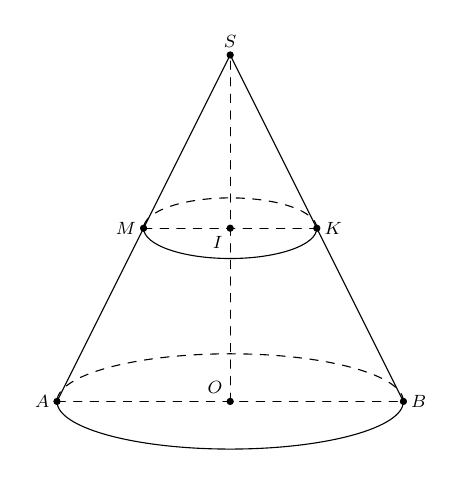
\begin{tikzpicture}[scale=1.1,font=\footnotesize,line join=round, line cap=round,>=stealth]
			\draw[black] (0,0)arc(0:-180:2 and 0.55);
			\draw[black] (-1,2)arc(0:-180:1 and 0.35);
			\draw[dashed] (0,0)arc(0:180:2 and 0.55);
			\draw[dashed] (-1,2)arc(0:180:1 and 0.35);
			\draw[dashed] (-4,0)--(0,0) (-2,0) node[above left,scale = 0.8]{$O$} -- (-2,2) node[below left,scale = 0.8]{$I$}--(-2,4) node[above,scale = 0.8]{$S$};
			\draw[dashed] (-3,2) node[left,scale = 0.8]{$M$}--(-1,2)  node[right,scale = 0.8]{$K$};
			\draw (-4,0) node[left,scale = 0.8]{$A$}--(-2,4)--(0,0) node[right,scale = 0.8]{$B$};
			\draw[fill = black] (0,0)circle (1pt) (-4,0)circle (1pt) (-2,4) circle (1pt) (-2,2) circle (1pt) (-3,2) circle (1pt) (-1,2) circle (1pt) (-2,0) circle (1pt);
			\end{tikzpicture}
		}
		\noindent 		Thể tích khối nón $(N)$ là $V_{(N)}=\dfrac{1}{3}\cdot\pi\cdot r_2^2\cdot h_2 =\dfrac{1}{3}\cdot\pi\cdot\left(\dfrac{12}{5}\right)^2\cdot\dfrac{16}{5} =\dfrac{768}{125}\pi$ cm$^3$.	
	}
\end{ex}

\begin{ex}%[2H2B1-1]%[Thành Đức Trung]%Câu 20.
	Cho một khối nón có bán kính đáy là $9$ cm, góc giữa đường sinh và mặt đáy là $30^{\circ}$. Tính diện tích thiết diện của khối nón cắt bởi mặt phẳng đi qua hai đường sinh vuông góc với nhau. 
	\choice
	{$27\left(\text{cm}^2\right)$}
	{$162\left(\text{cm}^2\right)$}
	{$\dfrac{27}{2}\left(\text{cm}^2\right)$}
	{\True $54\left(\text{cm}^2\right)$}
	\loigiai{
		\immini{
			Mặt phẳng đi qua hai đường sinh vuông góc là $SA$ và $AM$ cắt khối nón theo thiết diện là tam giác $SAM$.\\
			Góc giữa đường sinh và mặt đáy là $\widehat{SAO}=30^{\circ}$.\\
			Ta có $SM=SA=\dfrac{r}{\cos 30^{\circ}} =\dfrac{9}{\dfrac{\sqrt{3}}{2}}=6\sqrt{3}$.\\
			Vì $SA\perp AM$ nên tam giác $SAM$ vuông tại $S$.\\
			Do đó diện tích tam giác $SAM$ là $S=\dfrac{1}{2}SA\cdot SM= 54\left(\text{cm}^2\right)$.
		}{
			\begin{tikzpicture}[scale=0.45]
			\tkzSetUpPoint[color=black,fill=black]
			\tkzDefPoint(0,0){O}
			\pgfmathsetmacro{\a}{5}
			\pgfmathsetmacro{\b}{1.3} 
			\tkzDefPoint(\a,0){E}
			\draw[smooth,dashed,samples=200,variable=\t,domain=20:160] plot({\a*cos (\t)},{\b*sin(\t)});
			\draw[smooth,samples=200,variable=\t,domain=160:380] plot({\a*cos (\t)},{\b*sin(\t)});
			\tkzDefPointWith[orthogonal,K=1.5](O,E)
			\tkzGetPoint{S}
			\tkzDefPoint({\a*cos(-20/180*pi)},{\b*sin(-20/180*pi)}){A}
			\tkzDefPointBy[symmetry =center O](A)
			\tkzGetPoint{A1}
			\tkzDefPoint({\a*cos(20*pi/180)},{\b*sin(20*pi/180)}){A2}
			\tkzDefPoint({\a*cos(-120*pi/180)},{\b*sin(-120*pi/180)}){B}
			\tkzDrawSegments(S,A S,B S,A1 S,A2)
			\tkzDrawSegments[dashed](A,A1 S,O B,A O,B)
			\tkzDrawPoints[fill = black, size = 2](O,S,A,B)
			\tkzLabelPoint[above left](O){\footnotesize $O$}
			\tkzLabelPoint[below](A){\footnotesize $A$}
			\tkzLabelPoint[above](S){\footnotesize $S$}
			\tkzLabelPoint[below](B){\footnotesize $M$}
			\tkzLabelPoint[above left](A1){\footnotesize $B$}
			\tkzLabelSegment[above,rotate=-6](O,A){\footnotesize $r=9$cm}
			\end{tikzpicture}
		}	
	}
\end{ex}

\begin{ex}%[2H2Y1-1]%[Thành Đức Trung]%Câu 21.
	Cho khối nón có bán kính đáy $R$, độ dài đường sinh $\ell$. Thể tích khối nón là
	\choice
	{$\dfrac{1}{3}\pi R^2\ell$}
	{$\pi R^2\ell$}
	{\True $\dfrac{1}{3}\pi R^2\sqrt{\ell^2-R^2}$}
	{$\pi R^2\sqrt{\ell^2-R^2}$}
	\loigiai{
		Đường cao khối nón $h=\sqrt{\ell^2-R^2}$.\\
		Thể tích khối nón $V=\dfrac{1}{3}Sh =\dfrac{1}{3}\pi R^2\sqrt{\ell^2-R^2}$.}
\end{ex}

\begin{ex}%[2H2B2-2]%[Thành Đức Trung]%Câu 22.
	Cho hình lập phương có cạnh bằng $1$. Diện tích của mặt cầu ngoại tiếp hình lập phương đó bằng
	\choice
	{\True $3\pi$}
	{$12\pi$}
	{$\pi$}
	{$6\pi$}
	\loigiai{
		\immini{
			Đường chéo hình lập phương bằng $\sqrt{1^2+1^2+1^2}=\sqrt{3}$.\\
			Bán kính mặt cầu ngoại tiếp hình lập phương là $R=\dfrac{\sqrt{3}}{2}$.\\
			Diện tích của mặt cầu ngoại tiếp hình lập phương đó bằng $S=4\pi R^2 =4\pi\left(\dfrac{\sqrt{3}}{2}\right)^2=3\pi$.
		}{
			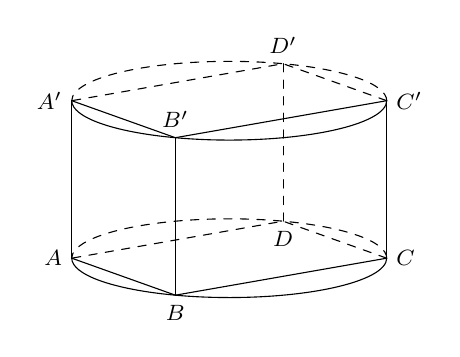
\begin{tikzpicture}[scale=1, font=\footnotesize, line join=round, line cap=round, >=stealth]
			\def\r{0.5}
			\def\goc{70}
			\draw (-2,0)coordinate (A) node[left]{$A$}
			arc (180:180+\goc:2 and \r)coordinate (B) node[below]{$B$}
			arc (180+\goc:360:2 and \r);
			\draw[dashed] (2,0)coordinate (C) node[right]{$C$}
			arc (0:\goc:2 and \r)coordinate (D) node[below]{$D$}
			arc (\goc:180:2 and \r);
			\draw (A)--(B)--(C);
			\draw[dashed] (C)--(D)--(A);
			\begin{scope}[yshift=2cm]
			\draw (-2,0)coordinate (A') node[left]{$A'$}
			arc (180:180+\goc:2 and \r)coordinate (B') node[above]{$B'$}
			arc (180+\goc:360:2 and \r);
			\draw[dashed] (2,0)coordinate (C') node[right]{$C'$}
			arc (0:\goc:2 and \r)coordinate (D') node[above]{$D'$}
			arc (\goc:180:2 and \r);
			\draw (A')--(B')--(C');
			\draw[dashed] (C')--(D')--(A');
			\end{scope}
			\tkzDrawCircle[circum](A,C,C')
			\draw (A)--(A') (B)--(B') (C)--(C');
			\draw[dashed] (D)--(D');
			\end{tikzpicture}
		}	
	}
\end{ex}

\begin{ex}%[2H2B1-2]%[Thành Đức Trung]%Câu 23.
	Cho hình lập phương $ABCD.A'B'C'D'$ có cạnh $a$. Một khối nón có đỉnh là tâm của hình vuông $ABCD$ và đáy là hình tròn nội tiếp hình vuông $A'B'C'D'$. Kết quả tính diện tích toàn phần $S_{\text{tp}}$ của khối nón đó có dạng bằng $\dfrac{\pi a^2}{4}\left(\sqrt{b}+c\right)$ với $b$ và $c$ là hai số nguyên dương và $b>1$. Tính $bc$. 
	\choice
	{\True $bc=5$}
	{$bc=8$}
	{$bc=15$}
	{$bc=7$}
	\loigiai{
		\immini{
			Ta có bán kính hình nón $r=\dfrac{a}{2}$, đường cao $h=a$, đường sinh $\ell=\dfrac{a\sqrt{5}}{2}$.\\
			Diện tích toàn phần $S_{\text{tp}} =\pi r\ell+\pi r^2 =\pi\dfrac{a^2\sqrt{5}}{4}+\pi\dfrac{a^2}{4} =\dfrac{\pi a^2}{4}\left(\sqrt{5}+1\right)$.\\
			$\Rightarrow b=5$, $c=1$.\\
			Vậy $bc=5$.
		}{
			\begin{tikzpicture}[scale=0.8, line join=round, line cap=round]
			\tkzDefPoints{0/0/A,-1.3/-1.1/B,2/-1.1/C}
			\coordinate (D) at ($(A)+(C)-(B)$);
			\coordinate (A') at ($(A)+(0,2.5)$);
			\tkzDefPointsBy[translation=from A to A'](B,C,D){B'}{C'}{D'}
			\coordinate (S) at ($(A')!1/2!(C')$);
			\coordinate (O) at ($(A)!1/2!(C)$);
			\coordinate (M) at ($(A)!1/2!(B)$);
			\coordinate (N) at ($(D)!1/2!(C)$);
			\coordinate (P) at ($(D)!1/2!(A)$);
			\tkzDrawPolygon(A',B',B,C,D,D')
			\tkzDrawSegments(B',C' C',D' C,C' A',C' B',D' A',B' A',D' B,B' B,C C,D D,D')
			\tkzDrawSegments[dashed](A,B A,D A,A' S,O S,M S,N)	
			\draw[dashed] (N) arc (0:180:1.59cm and 0.55cm);
			\draw[dashed] (M) arc (180:360:1.59cm and 0.55cm);
			\tkzDrawPoints[fill=black,size=2](A,B,D,C,A',B',C',D',S,O)	
			\tkzLabelPoints[above, scale = 0.75](A',B',C',D');	
			\tkzLabelPoints[below, scale = 0.75](A,B,C,D)
			\end{tikzpicture}
		}	
	}
\end{ex}

\begin{ex}%[2H2B1-1]%[Thành Đức Trung]%Câu 24.
	Cho hình nón có bán kính đáy bằng $2$ (cm), góc ở đỉnh bằng $60^{\circ}$. Thể tích khối nón là
	\choice
	{$V=\dfrac{8\pi\sqrt{3}}{9}\left(\text{cm}^3\right)$}
	{$V=\dfrac{8\pi\sqrt{3}}{2}\left(\text{cm}^3\right)$}
	{$V=8\pi\sqrt{3}\left(\text{cm}^3\right)$}
	{\True $V=\dfrac{8\pi\sqrt{3}}{3}\left(\text{cm}^3\right)$}
	\loigiai{
			Ta có bán kính đáy $r=2$, đường cao $h=\dfrac{r}{\tan 30^{\circ}}\Rightarrow h=2\sqrt{3}$.\\
			Vậy thể tích khối nón $V=\dfrac{1}{3}\pi r^2h =\dfrac{1}{3}\pi\cdot 4\cdot 2\sqrt{3} =\dfrac{8\pi\sqrt{3}}{3}\left(\text{cm}^3\right)$.
			\begin{center}
				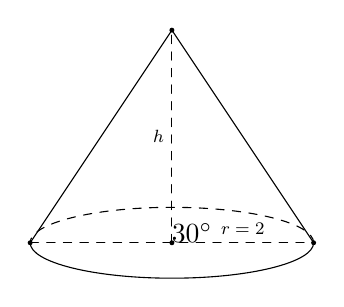
\begin{tikzpicture}[scale=0.9, font=\footnotesize, line join=round, line cap=round, >=stealth]
			\coordinate (O) at (0,0);\coordinate (S) at (0,3);\coordinate (B) at (2,0);
			\draw[dashed] (2,0) arc [start angle=0,end angle=180, x radius=2,y radius=1/2];
			\draw (-2,0) arc [ start angle=180, end angle=360, x radius=2,y radius=1/2];
			\draw[dashed] (-2,0)--(2,0) node[pos=0.75,above,scale = 0.8]{$ r=2 $};
			\draw [dashed] (0,0)--(0,3) node[pos=0.5,left,scale = 0.8]{$ h $};
			\draw (-2,0)--(0,3);\draw (0,3)--(2,0);
			\fill (0,0) circle(1pt) (-2,0) circle(1pt) (2,0) circle(1pt) (0,3) circle(1pt);
			\tkzLabelAngle[scale=0.75](O,S,B){$30^\circ$};
			\tkzMarkAngle[scale=0.65](O,S,B);
			\end{tikzpicture}
			\end{center}
	}
\end{ex}

\begin{ex}%[2H2Y1-1]%[Thành Đức Trung]%Câu 25.
	Mặt phẳng đi qua trục hình trụ, cắt hình trụ theo thiết diện là hình vuông cạnh bằng $a$. Thể tích khối trụ đó bằng
	\choice
	{$\pi a^3$}
	{$\dfrac{\pi a^3}{2}$}
	{$\dfrac{\pi a^3}{3}$}
	{\True $\dfrac{\pi a^3}{4}$}
	\loigiai{
			Bán kính của đường tròn đáy là $r=\dfrac{a}{2}$.\\
			Chiều cao của hình trụ là $h=a$.\\
			Thể tích của khối trụ là $V=\pi r^2h =\pi\cdot\left(\dfrac{a}{2}\right)^2\cdot a =\dfrac{\pi a^3}{4}$.
			\begin{center}
				\begin{tikzpicture}[scale=0.7, font=\footnotesize, line join=round, line cap=round, >=stealth]
			\tikzset{label style/.style={font=\footnotesize}}
			\tkzDefPoints{0/0/O}
			\tkzDefShiftPoint[O](-120:2){A}
			\tkzDefShiftPoint[O](120:2){B}
			\tkzDefShiftPoint[O](60:2){C}
			\tkzDefShiftPoint[O](-60:2){D}
			\draw (D) arc (0:-180:2cm and 1cm);
			\draw[dashed] (D) arc (0:180:2cm and 1cm);
			\draw (C) arc (0:-360:2cm and 1cm);
			\coordinate (C') at ($2*(B)-(C)$);
			\coordinate (D') at ($2*(A)-(D)$);	
			\tkzDrawPoints[size=2](A,B,C,D)
			\tkzDrawSegments(C,C' C',D' C,D)
			\tkzDrawSegments[dashed](D,D')
			\tkzLabelSegment[right](C,D){$h=a$}
			\tkzLabelSegment[above](C',C){$a$}
			\tkzMarkRightAngle(A,D,C);
			\end{tikzpicture}
			\end{center}
	}
\end{ex}
\setcounter{ex}{25}
\begin{ex}%[2H2B1-2]%Câu 26.
	Một tứ diện đều cạnh $a$ có một đỉnh trùng với đỉnh hình nón, ba đỉnh còn lại nằm trên đường tròn đáy của hình nón. Khi đó diện tích xung quanh của hình nón bằng
	\choice
	{$\dfrac{\sqrt{3}}{2}\pi a^2$}
	{$\dfrac{2\sqrt{3}}{3}\pi a^2$}
	{\True $\dfrac{\sqrt{3}}{3}\pi a^2$}
	{$\sqrt{3}\pi a^2$}
	\loigiai{
	\begin{center}
		\begin{tikzpicture}
		\tkzDefPoints{0/0/O, 5/0/B, -5/0/M, 0/8/A}
		\coordinate (C) at ($(O)+({5*cos (-110)},{0.9*sin(-110)})$);
		\coordinate (D) at ($(O)+({5*cos (-120)},{0.9*sin(120)})$);
		\draw (5,0) arc (0:-180: 5 and 0.9);
		\draw[dashed] (5,0) arc (0:180: 5 and 0.9);
		\tkzDrawPoints(A,B,O,C,D)
		\draw[dashed] (A)--(O) (B)--(C)--(D)--(B) (D)--(A)--(C);
		\draw (M)--(A)--(B) ;
		\tkzLabelPoints[above right](D)
		\tkzLabelPoints[below left](C)
		\tkzLabelPoints[below right](B)
		\tkzLabelPoints[above](A)
		\tkzLabelPoints[above left](O)
		\end{tikzpicture}
	\end{center}
		Gọi tứ diện đều cạnh $a$ là $ABCD$, $O$ là tâm đường tròn đáy của hình nón.\\
		Diện tích xung quanh của hình nón là $S_{xq}=\pi rl =\pi\cdot BO\cdot AD =\pi\cdot\left(\dfrac{2}{3}\cdot\dfrac{a\sqrt{3}}{2}\right)\cdot a =\dfrac{\sqrt{3}}{3}\pi a^2$.}
\end{ex}
\begin{ex}%[2H2B1-1]%Câu 27.
	Cho hình nón có chiều cao bằng $3$ (cm), góc giữa trục và đường sinh bằng $60^{\circ}$. Thể tích khối nón bằng
	\choice
	{$V=9\pi\left(cm^3\right)$}
	{$V=54\pi\left(cm^3\right)$}
	{$V=18\pi\left(cm^3\right)$}
	{\True $V=27\pi\left(cm^3\right)$}
	\loigiai{
		Gọi $R$ là bán kính của hình nón. Khi đó, ta có $\tan 60^{\circ}=\dfrac{R}{3}\Rightarrow R=3\cdot\tan 60^{\circ}=3\sqrt{3}$.\\
		Vậy thể tích khối nón bằng $V=\dfrac{1}{3}\cdot\pi\cdot R^2\cdot h=\dfrac{1}{3}\cdot\pi\cdot(3\sqrt{3})^2\cdot 3=27\pi\left(cm^3\right)$.}
\end{ex}
\begin{ex}%[2H2B2-1]%Câu 28.
	Quay một miếng bìa hình tròn có diện tích $16\pi a^2$ quanh một trong những đường kính, ta được khối tròn xoay có thể tích là
	\choice
	{$\dfrac{64}{3}\pi a^3$}
	{$\dfrac{128}{3}\pi a^3$}
	{\True $\dfrac{256}{3}\pi a^3$}
	{$\dfrac{32}{3}\pi a^3$}
	\loigiai{
		Gọi $R$ là bán kính đường tròn. Theo giả thiết, ta có $S=\pi R^2=16\pi a^2\Rightarrow R=4a$.\\
		Khi quay miếng bìa hình tròn quanh một trong những đường kính của nó thì ta được một khối cầu. Thể tích khối cầu này là $V=\dfrac{4}{3}\cdot\pi\cdot R^3=\dfrac{4}{3}\cdot\pi\cdot(4a)^3=\dfrac{256}{3}\pi a^3$.}
\end{ex}
\begin{ex}%[2H2B1-3]%Câu 29.
	Cho lăng trụ đứng $ABC.A'B'C'$ có độ dài cạnh bên bằng $2a$, đáy $ABC$ là tam giác vuông cân tại $A$, góc giữa $AC'$ và mặt phẳng $(BCC'B')$ bằng $30^{\circ}$ (tham khảo hình vẽ). Thể tích của khối trụ ngoại tiếp lăng trụ $ABC.A'B'C'$ bằng\\
	\begin{center}
		\begin{tikzpicture}[scale=1]
		\tkzDefPoints{0/0/O, 3/0/C, -3/0/B, 0/3/O', -3/3/B', 3/3/C'}
		\draw (3,0) arc (0:-180: 3 and 0.9);
		\draw[dashed] (3,0) arc (0:180: 3 and 0.9);
		\coordinate (A) at ($(O)+({3*cos (80)},{0.9*sin(-80)})$);
		\coordinate (A') at ($(O')+({3*cos (80)},{0.9*sin(-80)})$);
		\draw(3,3) arc (0:360: 3 and 0.9);
		\tkzDrawPoints(A,B,C,A',B',C')
		\draw[dashed](B)--(C)--(A)--(B) (O)--(O') (A)--(C') (A)--(O)--(C');
		\draw (A)--(A')--(B')--(C')--(C) (B)--(B');
		\tkzLabelPoints[below left](A,O,A')
		\tkzLabelPoints[left](B')
		\tkzLabelPoints[right](C')
		\tkzLabelPoints[above left](B,O')
		\tkzLabelPoints[above right](C)
		\end{tikzpicture}
	\end{center}
	\choice
	{$\pi a^3$}
	{$2\pi a^3$}
	{\True $4\pi a^3$}
	{$3\pi a^3$}
	\loigiai{
		Gọi bán kính của hình trụ là $R$.\\
		Ta có: $CC'\perp(ABC)\Rightarrow CC'\perp AO$.\\
		Lại có tam giác $ABC$ là tam giác vuông cân tại $A$ nên $AO\perp BC$ do đó $AO\perp(BCC'B')$ hay góc giữa $AC'$ và mặt phẳng $(BCC'B')$ là $\widehat{OC'A}$.\\
		Xét tam giác $AOC'$ ta có: $OC'=\dfrac{AO}{\tan\widehat{OC'A}} =R\sqrt{3}$.\\
		Xét tam giác $COC'$ ta có: $OC'^2=OC^2+CC'^2\Leftrightarrow 3R^2=R^2+4a^2\Rightarrow R=a\sqrt{2}$.\\
		Thể tích khối trụ ngoại tiếp lăng trụ $ABC.A'B'C'$ là $V=\pi R^2\cdot h =4\pi a^3$.}
\end{ex}
\begin{ex}%[2H2B2-2]%Câu 30.
	Tính diện tích $S$ của mặt cầu ngoại tiếp hình chóp $S.ABC$ có $SA=6$, $SB=8$, $SC=10$ và $SA$, $SB$, $SC$ đôi một vuông góc. 
	\choice
	{$S=100\pi$}
	{$S=400\pi$}
	{\True $S=200\pi$}
	{$S=150\pi$}
	\loigiai{
		\begin{center}
			\begin{tikzpicture}
		\tkzDefPoints{-2/4/A,-2/0/S,0/-2/B, 3/1/C}
		\tkzDefMidPoint(B,C)
		\tkzGetPoint{M}
		\tkzDefMidPoint(S,A)
		\tkzGetPoint{N}
		\tkzDefLine[parallel=through N](S,M)
		\tkzGetPoint{c}
		\tkzDefLine[parallel=through M](S,A)
		\tkzGetPoint{d}
		\tkzInterLL(N,c)(M,d)
		\tkzGetPoint{I}
		\tkzInterLL(N,c)(A,M)
		\tkzGetPoint{K}
		\tkzDrawSegments(S,A A,B B,C S,B A,C A,M M,I K,I M,d)
		\tkzDrawSegments[dashed](S,M S,C N,K)
		\tkzLabelPoints(B,C,M,I)
		\tkzLabelPoints[left](S,A,N)
		\tkzLabelSegment[right,pos=0.9](M,d){$d$}
		\end{tikzpicture}
		\end{center}
		Ta có bán kính mặt cầu ngoại tiếp hình chóp $SO=\dfrac{1}{2}\sqrt{SA^2+SB^2+SC^2} =5\sqrt{2}$.\\
		Diện tích mặt cầu $S=4\pi R^2=200\pi$.}
\end{ex}
\begin{ex}%[2H2B1-1]%Câu 31.
	Cắt hình nón bởi một mặt phẳng đi qua trục ta được thiết diện là một tam giác vuông cân có cạnh huyền bằng $a\sqrt{6}$. Tính thể tích $V$ của khối nón đó. 
	\choice
	{\True $V=\dfrac{\pi a^3\sqrt{6}}{4}$}
	{$V=\dfrac{\pi a^3\sqrt{6}}{2}$}
	{$V=\dfrac{\pi a^3\sqrt{6}}{6}$}
	{$V=\dfrac{\pi a^3\sqrt{6}}{3}$}
	\loigiai{
		\begin{center}
			\begin{tikzpicture}[scale=0.9]
		\tkzDefPoints{0/0/O, 3/0/B, -3/0/A, 0/4/S}
		\draw (3,0) arc (0:-180: 3 and 0.7);
		\draw[dashed] (3,0) arc (0:180: 3 and 0.7);
		\tkzDrawPoints(A,B,S,O)
		\draw[dashed](A)--(B) (S)--(O);
		\draw (A)--(S)--(B);
		\tkzLabelPoints[below left](A,O)
		\tkzLabelPoints[below right](B)
		\tkzLabelPoints[above](S)
		\end{tikzpicture}
		\end{center}
		Khối nón có $2r=a\sqrt{6}\Leftrightarrow r=\dfrac{a\sqrt{6}}{2}$ và $h=r$ suy ra thể tích $V=\dfrac{1}{3}\pi r^2h=\dfrac{\pi a^3\sqrt{6}}{4}$.}
\end{ex}
\begin{ex}%[2H2B1-1]%Câu 32.
	Trong không gian cho tam giác $ABC$ vuông tại $A$ có $AB=\sqrt{3}$ và $\widehat{ACB}=30^{\circ}$. Tính thể tích $V$ của khối nón nhận được khi quay tam giác $ABC$ quanh cạnh $AC$. 
	\choice
	{$V=5\pi$}
	{$V=9\pi$}
	{\True $V=3\pi$}
	{$V=2\pi$}
	\loigiai{
		Xét tam giác vuông $ABC$ ta có $AC=\dfrac{AB}{\tan 30^{\circ}}=3$.\\
		Thể tích của khối nón nhận được khi quay tam giác $ABC$ quanh cạnh $AC$ là $V=\dfrac{1}{3}\pi AB^2\cdot AC=3\pi$.}
\end{ex}
\begin{ex}%[2H2K1-2]%Câu 33.
	Cho hình chóp tứ giác đều $S.ABCD$ có tất cả các cạnh bằng $3$. Tính diện tích xung quanh của hình nón có đáy là đường tròn ngoại tiếp tứ giác $ABCD$ và chiều cao bằng chiều cao của hình chóp. 
	\choice
	{$S_{xq}=\dfrac{9\pi}{2}$}
	{$S_{xq}=\dfrac{9\sqrt{2}\pi}{4}$}
	{$S_{xq}=9\pi$}
	{\True $S_{xq}=\dfrac{9\sqrt{2}\pi}{2}$}
	\loigiai{
		\begin{center}
			\begin{tikzpicture}[line cap=round,line join=round]%[Đức Nguyễn]
			\def \x{0}%Hoành độ tâm I
			\def \y{0}%Tung độ tâm I
			\def \z{6}%Chiều cao
			\def \a{3.9}%Trục lớn
			\def \b{1}%Trục nhỏ
			\coordinate (O) at (\x,\y);
			\coordinate (S) at ($(O) + (0,\z)$);
			%\draw (I) ellipse (\a cm and \b cm);
			\coordinate (M) at ($(O) + (-\a,0)$);
			\coordinate (G) at ($(O) + (0,\b)$);
			\coordinate (N) at ($(O) + (\a,0)$);
			\coordinate (B) at ($(O) + (-70:{\a} and {\b})$);
			\coordinate (C) at ($(O) + (40:{\a} and {\b})$);
			\draw[dashed] (M) arc (180:0:{\a} and {\b});
			\draw (N) arc (360:0:{\a} and {\b});
			\tkzDefPointBy[symmetry = center O](B)
			\tkzGetPoint{D}
			\tkzDefPointBy[symmetry = center O](C)
			\tkzGetPoint{A}
			\tkzDrawPoints[fill=black](S,O,B)
			\tkzDrawSegments(S,M)% nối SA
			\tkzDrawSegments(S,N)
			\tkzDrawSegments[dashed](S,O)%nối OS nét đứt
			\tkzDrawSegments(S,M)
			\tkzDrawSegments[dashed](S,C)
			\tkzDrawSegments[dashed](O,B)
			\tkzLabelPoints[below](O)
			\tkzLabelPoints[below](B)
			\tkzLabelPoints[above](S)
			\tkzLabelPoints[above](C)
			\tkzDrawSegments[dashed](C,B)
			\tkzDrawSegments[dashed](O,C)	
			\tkzLabelPoints[below](A)
			\tkzLabelPoints[above](D)
			\tkzDrawSegments[dashed](A,B)
			\tkzDrawSegments[dashed](A,D)
			\tkzDrawSegments[dashed](C,D)
			\tkzDrawSegments[dashed](S,D)
			\tkzDrawSegments (S,B)
			\tkzDrawSegments (S,A)
			\tkzDrawSegments[dashed](A,O)
			\tkzDrawSegments[dashed](D,O)
			\end{tikzpicture}
		\end{center}
		Hình nón có bán kính đáy là $r=\dfrac{1}{2}AC=\dfrac{3\sqrt{2}}{2}$.\\
		Độ dài đường sinh của hình nón là $l=SA=3$. Do đó $S_{xq}=\pi rl=\dfrac{9\sqrt{2}\pi}{2}$.}
\end{ex}
\begin{ex}%[2H2B2-3]%Câu 34.
	Cho hình lập phương có thể tích bằng $64a^3$. Thể tích của khối cầu nội tiếp của hình lập phương đó bằng
	\choice
	{$V=\dfrac{16\pi a^3}{3}$}
	{$V=\dfrac{64\pi a^3}{3}$}
	{\True $V=\dfrac{32\pi a^3}{3}$}
	{$V=\dfrac{8\pi a^3}{3}$}
	\loigiai{
		\begin{center}
			\begin{tikzpicture}
		\def\r{2}
		\def\g{-75}
		\pgfmathsetmacro{\a}{\r *sqrt(2)}
		\begin{scope}[y=.25cm]
		\path
		(0:0)coordinate(O)
		(\g:\a) coordinate (A)
		--(\g+90:\a) coordinate (B)
		--(\g+180:\a) coordinate (C)
		--(\g+270:\a) coordinate (D)
		(180:\r)coordinate(M)
		(0:\r) coordinate(N)
		;
		\draw (D)--(A)--(B);
		\draw[dashed] (D)--(C)--(B);
		\end{scope}
		\begin{scope}[shift={(0,2*\r)} ,y=.25cm]
		\path
		(0:0)coordinate (O')
		(\g:\a) coordinate (A')
		--(\g+90:\a) coordinate (B')
		--(\g+180:\a) coordinate (C')
		--(\g+270:\a) coordinate (D')
		(180:\r)coordinate(M')
		(0:\r) coordinate(N')
		;
		\draw (A')--(B')--(C')--(D')--(A');
		\end{scope}
		\draw[dashed] ($(O)!.5!(O')$) circle (\r);
		\foreach \x in {A,B,D}\draw (\x)--(\x');
		\foreach \x in {C,O}\draw[dashed](\x)--(\x');
		\foreach \x in {A,B,C,D,O}\fill[black](\x) circle (1pt) (\x') circle (1pt);
		\end{tikzpicture}
		\end{center}
		Khối lập phương có thể tích $64a^3$ nên cạnh bằng $4a$. Khối cầu nội tiếp hình lập phương có bán kính $R=\dfrac{4a}{2}=2a$ nên thể tích khối cầu $V=\dfrac{4}{3}\pi R^3=\dfrac{4}{3}\pi(2a)^3=\dfrac{32\pi a^3}{3}$.}
\end{ex}
\begin{ex}%[2H2B1-3]%Câu 35.
	Một hình trụ có thiết diện qua trục là hình vuông, diện tích xung quanh bằng $36\pi a^2$. Tính thể tích $V$ của lăng trụ lục giác đều nội tiếp hình trụ. 
	\choice
	{$V=27\sqrt{3}a^3$}
	{\True $V=81\sqrt{3}a^3$}
	{$V=24\sqrt{3}a^3$}
	{$V=36\sqrt{3}a^3$}
	\loigiai{
		\begin{center}
			\begin{tikzpicture}[scale=0.6]
			\tkzDefPoints{0/0/O, 3/0/C, -3/0/B, 0/6/O', -3/6/B', 3/6/C'}
			\draw (3,0) arc (0:-180: 3 and 0.9);
			\draw[dashed] (3,0) arc (0:180: 3 and 0.9);
			\coordinate (A) at ($(O)+({3*cos (50)},{0.9*sin(-50)})$);
			\coordinate (E) at ($(O)+({3*cos (-60)},{0.9*sin(60)})$);
			\coordinate (D) at ($(O)+({3*cos (110)},{0.9*sin(-110)})$);
			\coordinate (F) at ($(O)+({3*cos (-120)},{0.9*sin(120)})$);
			\coordinate (A') at ($(O')+({3*cos (50)},{0.9*sin(-50)})$);
			\coordinate (E') at ($(O')+({3*cos (-60)},{0.9*sin(60)})$);
			\coordinate (D') at ($(O')+({3*cos (110)},{0.9*sin(-110)})$);
			\coordinate (F') at ($(O')+({3*cos (-120)},{0.9*sin(120)})$);
			\draw(3,6) arc (0:360: 3 and 0.9);
			\tkzDrawPoints(A,B,C,D,E,F,A',B',C',D',E',F',O,O')
			\draw[dashed](B)--(D)--(A)--(C)--(E)--(F)--(B) (O)--(O') (E)--(E') (F)--(F') (B)--(C);
			\draw (A)--(A') (B')--(C')--(C) (B)--(B') (D)--(D') (B')--(D')--(A')--(C')--(E')--(F')--(B');
			\end{tikzpicture}
		\end{center}
		Diện tích xung quanh hình trụ $S_{xq}=2\pi rl =2\pi r\cdot 2r=36\pi a^2\Rightarrow r=3a$.\\
		Lăng trụ lục giác đều có đường cao $h=l=6a$.\\
		Lục giác đều nội tiếp đường tròn có cạnh bằng bán kính của đường tròn.\\
		Suy ra diện tích lục giác đều $S=6\cdot\dfrac{(3a)^2\sqrt{3}}{4} =\dfrac{27a^2\sqrt{3}}{2}$. Vậy thể tích $V=S\cdot h=81\sqrt{3}a^3$.}
\end{ex}
\begin{ex}%[2H2B2-2]%Câu 36.
	Cho khối chóp $S.ABC$ có đáy là tam giác vuông tại $B$, $AB=1$, $BC=\sqrt{2}$, cạnh bên $SA$ vuông góc với đáy và $SA=\sqrt{3}$. Diện tích mặt cầu ngoại tiếp hình chóp $S.ABC$ bằng
	\choice
	{\True $6\pi$}
	{$\dfrac{3\pi}{2}$}
	{$12\pi$}
	{$2\pi$}
	\loigiai{
		\begin{center}
			\begin{tikzpicture}
		\tkzDefPoints{-2/4/S, -2/0/A,0/-2/B, 3/0/C}
		\tkzDefMidPoint(S,C)
		\tkzGetPoint{I}
		\tkzDrawSegments(S,A A,B B,C C,S S,B B,I)
		\tkzDrawSegments[dashed](A,C I,A)
		\tkzLabelPoints(B,C)
		\tkzLabelPoints[left](A)
		\tkzLabelPoints[right](I)
		\tkzLabelPoints[above](S)
		\end{tikzpicture}
		\end{center}
		Gọi $I$ là trung điểm của $SC$. Tam giác $SAC$ vuông tại $A\Rightarrow IA=IS=IC=\dfrac{1}{2}SC (1)$.\\
		Dễ dàng chứng minh được $BC\perp(SAB)\Rightarrow BC\perp SB$ hay tam giác $SBC$ vuông tại $B$ \\
		$ \Rightarrow IB=IS=IC=\dfrac{1}{2}SC (2) $.\\
		Từ $(1)$ và $(2)$ suy ra: $IA=IB=IC=IS=\dfrac{1}{2}SC$ hay $I$ là tâm mặt cầu ngoại tiếp hình chóp $S.ABC$ có bán kính $R=\dfrac{1}{2}SC=\dfrac{1}{2}\sqrt{SA^2+AC^2}=\dfrac{1}{2}\sqrt{SA^2+AB^2+BC^2}=\dfrac{\sqrt{6}}{2}$.\\
		Vậy diện tích mặt cầu cần tìm là $S=4\pi R^2=6\pi$.}
\end{ex}
\begin{ex}%[2H2B2-6]%Câu 37.
	\immini{Trong một chiếc hộp hình trụ người ta bỏ vào đó ba quả bóng tennis, biết rằng đáy của hình trụ bằng hình tròn lớn trên quả bóng và chiều cao của hình trụ bằng 3 lần đường kính của quả bóng. Gọi $S_1$ là tổng diện tích của ba quả bóng và $S_2$ là diện tích xung quanh của hình trụ. Giá trị biểu thức $2018^{\tfrac{S_1}{S_2}}$ bằng
	\choice
	{\True $2018$}
	{$1$}
	{$2018^{\pi}$}
	{$2018^{\sqrt{2}}$}
	}{\begin{tikzpicture}[ball/.style={circle, minimum size=25pt, draw}]
	\node (b1) [ball] {};
	\node (b2) [ball, below=0pt of b1] {};
	\node (b3) [ball, below=0pt of b2] {};
	\coordinate (c1) at ([yshift=6pt]b1.center);
	\node (c) [cylinder, draw, fit=(c1) (b2) (b3), shape border rotate=90, inner sep=0pt,, aspect=.5] {};
	\draw [<->] ([xshift=15pt]c.after top) coordinate (a1) -- ([xshift=15pt]c.before bottom) coordinate (a2) node [fill=white, midway] {$3d$};
	\draw [thin, draw=gray, densely dashed] (c.after top) -- (a1) (c.before bottom) -- (a2);
	\draw [thin, densely dashed, draw=gray] (c.before bottom) arc [x radius=12.5pt, y radius=6pt, start angle=0, end angle=180];
	\draw [thin, densely dashed, draw=gray] (b1.north) -- (b3.south) \foreach \i in {1,3,5} {node [left, pos=\i/6] {$d$}};
	\end{tikzpicture}}
	\loigiai{
		Giả sử bán kính quả bóng là $r$. Tổng diện tích ba quả bóng là $S_1=3\cdot 4\pi r^2=12\pi r^2$.\\
		Hình trụ có chiều cao $h=6r$, bán kính đường tròn đáy là $r$.\\
		Do đó $S_2=2\pi rh=12\pi r^2$. Vậy $2018^{\tfrac{S_1}{S_2}}=2018$.}
\end{ex}
\begin{ex}%[2H2B1-2]%Câu 38.
	Trong không gian cho hình chữ nhật $ABCD$ có $AB=a$ và $AD=2a$. Gọi $H$, $K$ lần lượt là trung điểm của $AD$ và $BC$. Quay hình chữ nhật đó quanh trục $HK$, ta được một hình trụ. Diện tích toàn phần của hình trụ là 
	\choice
	{$S_{tp}=8\pi$}
	{$S_{tp}=8a^2\pi$}
	{\True $S_{tp}=4a^2\pi$}
	{$S_{tp}=4\pi$}
	\loigiai{
		\immini
		{Quay hình chữ nhật $ABCD$ quanh trục $HK$ ta được hình trụ có đường cao là $h=AB=a$, bán kính đường tròn đáy là $R=BK=\dfrac{1}{2}BC=a$.\\
		Vậy diện tích toàn phần của hình trụ là $S_{tp}=2\pi Rh+2\pi R^2=4\pi a^2$.}
		{
			\begin{tikzpicture}[scale=0.6]
			\tkzDefPoints{0/0/H, 3/0/D, -3/0/A, 0/3/K, -3/3/B, 3/3/C}
			\draw (3,0) arc (0:-180: 3 and 0.9);
			\draw[dashed] (3,0) arc (0:180: 3 and 0.9);
			\draw(3,3) arc (0:360: 3 and 0.9);
			\tkzDrawPoints(A,B,H,K,C,D)
			\draw[dashed](A)--(D) (H)--(K);
			\draw (A)--(B)--(C)--(D);
			\tkzLabelPoints[below left](A,H)
			\tkzLabelPoints[below right](D)
			\tkzLabelPoints[above left](B,K)
			\tkzLabelPoints[above right](C)
			\end{tikzpicture}}}
\end{ex}
\begin{ex}%[2H2K1-3]%Câu 39.
	Cho hình nón $(N)$ có bán kính đáy bằng $a$ và diện tích xung quanh $S_{xp}=2\pi a^2$. Tính thể tích $V$ của khối chóp tứ giác đều $S.ABCD$ có đáy $ABCD$ nội tiếp đáy của khối nón $(N)$ và đỉnh $S$ trùng với đỉnh của khối nón $(N)$. 
	\choice
	{$V=\dfrac{2\sqrt{5}a^3}{3}$}
	{$V=\dfrac{2\sqrt{2}a^3}{3}$}
	{$V=2\sqrt{3}a^3$}
	{\True $V=\dfrac{2\sqrt{3}a^3}{3}$}
	\loigiai{
		\begin{center}
			\begin{tikzpicture}[line cap=round,line join=round]%[Đức Nguyễn]
			\def \x{0}%Hoành độ tâm I
			\def \y{0}%Tung độ tâm I
			\def \z{6}%Chiều cao
			\def \a{3.9}%Trục lớn
			\def \b{1}%Trục nhỏ
			\coordinate (O) at (\x,\y);
			\coordinate (S) at ($(O) + (0,\z)$);
			%\draw (I) ellipse (\a cm and \b cm);
			\coordinate (M) at ($(O) + (-\a,0)$);
			\coordinate (G) at ($(O) + (0,\b)$);
			\coordinate (N) at ($(O) + (\a,0)$);
			\coordinate (B) at ($(O) + (-70:{\a} and {\b})$);
			\coordinate (C) at ($(O) + (40:{\a} and {\b})$);
			\draw[dashed] (M) arc (180:0:{\a} and {\b});
			\draw (N) arc (360:0:{\a} and {\b});
			\tkzDefPointBy[symmetry = center O](B)
			\tkzGetPoint{D}
			\tkzDefPointBy[symmetry = center O](C)
			\tkzGetPoint{A}
			\tkzDrawPoints[fill=black](S,O,B)
			\tkzDrawSegments(S,M)% nối SA
			\tkzDrawSegments(S,N)
			\tkzDrawSegments[dashed](S,O)%nối OS nét đứt
			\tkzDrawSegments(S,M)
			\tkzDrawSegments[dashed](S,C)
			\tkzDrawSegments[dashed](O,B)
			\tkzLabelPoints[below](O)
			\tkzLabelPoints[below](B)
			\tkzLabelPoints[above](S)
			\tkzLabelPoints[above](C)
			\tkzDrawSegments[dashed](C,B)
			\tkzDrawSegments[dashed](O,C)	
			\tkzLabelPoints[below](A)
			\tkzLabelPoints[above](D)
			\tkzDrawSegments[dashed](A,B)
			\tkzDrawSegments[dashed](A,D)
			\tkzDrawSegments[dashed](C,D)
			\tkzDrawSegments[dashed](S,D)
			\tkzDrawSegments (S,B)
			\tkzDrawSegments (S,A)
			\tkzDrawSegments[dashed](A,O)
			\tkzDrawSegments[dashed](D,O)
			\end{tikzpicture}
		\end{center}
		Ta có: Diện tích xung quanh $S_{xp}=2\pi a^2\Rightarrow\pi rl=2\pi a^2\Rightarrow l=2a\Rightarrow h=\sqrt{l^2-r^2}=a\sqrt{3}$.\\
		Đáy $ABCD$ nội tiếp đáy của khối nón $(N)$ có bán kính đáy bằng $a\Rightarrow AB=a\sqrt{2}$.\\
		Vậy: $V=\dfrac{1}{3}S_{ABCD}h=\dfrac{2\sqrt{3}a^3}{3}$.}
\end{ex}
\begin{ex}%[2H2K1-3]%Câu 40.
	Cho hình nón đỉnh $S$, đáy là đường tròn nội tiếp tam giác $ABC$. Biết rằng $AB=BC=10a$, $AC=12a$, góc tạo bởi hai mặt phẳng $(SAB)$ và $(ABC)$ bằng $45^{\circ}$. Tính thể tích $V$ của khối nón đã cho. 
	\choice
	{$V=3\pi a^3$}
	{\True $V=9\pi a^3$}
	{$V=27\pi a^3$}
	{$V=12\pi a^3$}
	\loigiai{
		\begin{center}
			\begin{tikzpicture}[scale=0.8,>=stealth, font=\footnotesize, line join=round, line cap=round]
		\tkzDefPoints{0/0/B,6/0/C,2.1/-4/A,2.7/4/S}
		\coordinate (D) at ($(A)!0.5!(B)$);
		\coordinate (N) at ($(C)!0.5!(B)$);
		\coordinate (M) at ($(A)!0.5!(C)$);
		\tkzCentroid(A,B,C)\tkzGetPoint{G}
		\tkzDrawCircle[in,dashed](A,B,C)
		\tkzDrawSegments(A,C B,C S,A S,B S,C S,D)
		\tkzDrawSegments[dashed](B,A D,B S,G D,G)
		\tkzLabelPoints[below](A,G)
		\tkzLabelPoints[right](C)
		\tkzLabelPoints[left](B,D)
		\tkzLabelPoints[above](S)
		\end{tikzpicture}
		\end{center}
		Hạ $ID\perp AB$, khi đó góc tạo bởi hai mặt phẳng $(SAB)$ và $(ABC)$ chính là $\widehat{SDI}=45^{\circ}$ nên $ID=SI=r=h$.\\
		Lại có $S_{\triangle ABC}=p\cdot r\Rightarrow r=\dfrac{S_{\triangle ABC}}{p}$.\\
		Tính được $p=16a$, $S_{\triangle ABC}=\sqrt{p(p-a)(p-b)(p-c)}=48a^2$.\\
		Suy ra $r=3a$. Vậy $V=\dfrac{1}{3}\pi r^2h=\dfrac{1}{3}\pi(3a)^3=9\pi a^3$.}
\end{ex}
\begin{ex}%[2H2K1-5]%Câu 41.
	Cho tam giác $ABC$ vuông ở $A$ có $AB=2AC$. $M$ là một điểm thay đổi trên cạnh $BC$. Gọi $H$, $K$ lần lượt là hình chiếu vuông góc của $M$ trên $AB$, $AC$. Gọi $V$ và $V'$ tương ứng là thể tích của vật thể tròn xoay tạo bởi tam giác $ABC$ và hình chữ nhật $MHAK$ khi quay quanh trục $AB$. Tỉ số $\dfrac{V'}{V}$ lớn nhất bằng
	\choice
	{$\dfrac{1}{2}$}
	{\True $\dfrac{4}{9}$}
	{$\dfrac{2}{3}$}
	{$\dfrac{3}{4}$}
	\loigiai{
		\begin{center}
			
\begin{tikzpicture}[scale=0.8,>=stealth, font=\footnotesize, line join=round, line cap=round]
		\tkzDefPoints{0/0/A,6/0/B,0/3/C,4/1/M,0/1/K,4/0/H}
		\tkzDrawSegments(A,B B,C A,C M,H M,K)
		\tkzLabelPoints[left](A,C,K)
		\tkzLabelPoints[below](H,B)
		\tkzLabelPoints[above](M)
		\tkzLabelSegment(A,B){$2a$}
		\tkzLabelSegment(A,C){$a$}	
		\end{tikzpicture}
		\end{center}
		Giả sử $AC=a$, $AB=2a$, $BM=x$. Ta có:\\
		$BC=a\sqrt{5}$, $\sin\alpha=\dfrac{AC}{BC}=\dfrac{1}{\sqrt{5}}$, $\cos\alpha=\dfrac{2}{\sqrt{5}}$.\\
		$MH=x\sin\alpha=\dfrac{x}{\sqrt{5}}$, $HB=x\cos\alpha=\dfrac{2x}{\sqrt{5}}$, $AH=2a-\dfrac{2x}{\sqrt{5}}$.\\
		Khi quay tam giác $ABC$ quanh trục $AB$ ta được một khối nón có thể tích là\\
		$V=\dfrac{1}{3}\pi AC^2\cdot AB =\dfrac{2a^3\pi}{3}$.\\
		Khi quay hình chữ nhật $MHAK$ quanh trục $AB$ ta được một khối trụ có thể tích là\\
		$V'=\pi\cdot MH^2\cdot AH=\pi\dfrac{x^2}{5}\left(2a-\dfrac{2x}{\sqrt{5}}\right)$.\\
		Do đó, $\dfrac{V'}{V}=\dfrac{3}{5a^2}x^2-\dfrac{3}{5\sqrt{5}a^3}x^3$.\\
		Xét hàm số $f(x)=\dfrac{3}{5a^2}x^2-\dfrac{3}{5\sqrt{5}a^3}x^3$ trên đoạn $\left[0; a\sqrt{5}\right]$.\\
		Ta có: $f'(x)=\dfrac{6}{5a^2}x-\dfrac{9}{5\sqrt{5}a^3}x^2$; $f'(x)=0\Leftrightarrow\hoac{&x=0\\&x=\dfrac{2\sqrt{5}a}{3}\in[0;\sqrt{5}].}$ \\
		$f(0)=0$, $f(a\sqrt{5})=0$, $f\left(\dfrac{2a\sqrt{5}}{3}\right)=\dfrac{4}{9}$.\\
		Suy ra $\max\limits_{[0;\sqrt{5}]} f(x)=f\left(\dfrac{2a\sqrt{5}}{3}\right)=\dfrac{4}{9}$.\\
		Vậy giá trị lớn nhất của tỉ số $\dfrac{V'}{V}$ bằng $\dfrac{4}{9}$.}
\end{ex}
\begin{ex}%[2H2K1-4]%Câu 42.
	Mặt tiền của một ngôi biệt thự có $8$ cây cột hình trụ tròn, tất cả đều có chiều cao bằng $4,2$ m. Trong số các cây đó có $2$ cây cột trước đại sảnh đường kính bằng $40$ cm, $6$ cây cột còn lại phân bố đều hai bên đại sảnh và chúng đều có đường kính bằng $26$ cm. Chủ nhà thuê nhân công để sơn các cây cột bằng loại sơn giả đá, biết giá thuê là $380\cdot 000/m^2$ (kể cả vật liệu sơn và phần thi công). Hỏi người chủ phải chi ít nhất bao nhiêu tiền để sơn hết các cây cột nhà đó (đơn vị đồng)?\\
	(lấy $\pi\approx 3,14159$)
	\choice
	{$\approx 12\cdot 521\cdot 000$}
	{$\approx 15\cdot 642\cdot 000$}
	{$\approx 10\cdot 400\cdot 000$}
	{\True $\approx 11\cdot 833\cdot 000$}
	\loigiai{
		Các cây cột có chiều cao là $h=4,2$ m.\\
		$2$ cây cột trước đại sảnh bán kính bằng $R=0,2$ m.\\
		$6$ cây cột ở hai bên đại sảnh có bán kính bằng $r=0,13$ m.\\
		Diện tích xung quanh của $8$ cây cột là $S=4\pi Rh+12\pi rh =4\pi h(R+3r)\approx 31\cdot 13944008$.\\
		Số tiền ít nhất phải chi để sơn hết các cây cột là $S.380000\approx 11832987,23$.\\
		Vậy số tiền cần chi là $\approx 11\cdot 833\cdot 000$ đồng.}
\end{ex}
\begin{ex}%[2H2K1-3]%Câu 43.
	Cho hình chóp tứ giác đều $S.ABCD$ có cạnh đáy bằng $2a$. Mặt phẳng qua $AB$ và trung điểm $M$ của $SC$ cắt hình chóp theo thiết diện có chu vi bằng $7a$. Thể tích của khối nón có đỉnh là $S$ và đường tròn đáy ngoại tiếp tứ giác $ABCD$ bằng
	\choice
	{$\dfrac{2\pi a^3\sqrt{6}}{9}$}
	{$\dfrac{\pi a^3\sqrt{6}}{3}$}
	{$\dfrac{2\pi a^3\sqrt{3}}{3}$}
	{\True $\dfrac{2\pi a^3\sqrt{6}}{3}$}
	\loigiai{
		\begin{center}
			\begin{tikzpicture}[scale=1,>=stealth, font=\footnotesize, line join=round, line cap=round]
		\tkzDefPoints{0/0/A,-1.9/-1.6/B,1.6/-1.6/C}
		\coordinate (D) at ($(A)+(C)-(B)$);
		\coordinate (O) at ($(A)!1/2!(C)$);
		\coordinate (S) at ($(O)+(0,3.5)$);
		\coordinate (E) at ($(B)!1/2!(S)$);
		\coordinate (M) at ($(S)!1/2!(C)$);
		%\tkzDrawPolygon(S,B,C,D,E,M)
		\tkzDrawSegments(S,C S,B B,C C,D S,D E,M M,D)
		\tkzDrawSegments[dashed](A,S A,B A,D A,C B,D S,O A,E A,M)
		\tkzDrawPoints[fill=black,size=4](D,C,A,B,S,E,M)
		\tkzMarkRightAngles[size=0.16](A,O,B S,O,A S,O,B)
		\tkzLabelPoints[above](S)
		\tkzLabelPoints[below](A,C,O)
		\tkzLabelPoints[below left](B)
		\tkzLabelPoints[right](D,M)
		\tkzLabelPoints[left](E)
		\end{tikzpicture}
		\end{center}
		Gọi $E$ là trung điểm $SD\Rightarrow ME\parallel AB$ suy ra $(ABM)$ cắt hình chóp $S.ABCD$ theo thiết diện là hình thang $ABME$.\\
		Gọi độ dài cạnh bên của hình chóp là $x$. Do chóp $S.ABCD$ là chóp đều nên $\Delta SAD=\Delta SBC\Rightarrow AE=BM$.\\
		Áp dụng hệ thức trung tuyến ta có: $BM^2=\dfrac{SB^2+BC^2}{2}-\dfrac{SC^2}{4} =\dfrac{x^2+8a^2}{4}$.\\
		Suy ra $AE=BM =\sqrt{\dfrac{x^2+8a^2}{4}}$.\\
		Mặt khác dễ thấy $EM=a$, $AB=2a$ mà chu vi thiết diện bằng $7a$ nên ta có: $a+2a+2\sqrt{\dfrac{x^2+8a^2}{4}}=7a\Rightarrow x=2a\sqrt{2}$.\\
		Suy ra chiều cao của hình chóp: $SO^2=SA^2-\dfrac{AC^2}{4} =6a^2\Rightarrow SH=a\sqrt{6}$.\\
		Khối nón có đỉnh là $S$ và đường tròn đáy ngoại tiếp tứ giác $ABCD$ chiều cao là $SO=a\sqrt{6}$ và bán kính đường tròn đáy là $\dfrac{AC}{2}=a\sqrt{2}$ nên thể tích khối nón là\\
		$V=\dfrac{1}{3}\pi(a\sqrt{2})^2a\sqrt{6} =\dfrac{2\pi a^3\sqrt{6}}{3}$.}
\end{ex}
\begin{ex}%[2H2K2-3]%Câu 44.
	Cho hình chóp $S.ABC$ có đáy $ABC$ là tam giác vuông tại $B$, $BC=2a$. Mặt bên $(SAB)$ vuông góc với đáy, $\widehat{ASB}=60^{\circ}$, $SB=a$. Gọi $(S)$ là mặt cầu tâm $B$ và tiếp xúc với $(SAC)$. Tính bán kính $r$ của mặt cầu $(S)$. 
	\choice
	{$r=2a$}
	{\True $r=2a\sqrt{\dfrac{3}{19}}$}
	{$r=2a\sqrt{3}$}
	{$r=a\sqrt{\dfrac{3}{19}}$}
	\loigiai{
		\begin{center}
		\begin{tikzpicture}[scale=1,>=stealth, font=\footnotesize, line join=round, line cap=round]
		\tkzDefPoints{0/0/B,1.2/-1.5/A,4/0/S}
		\coordinate (C) at ($(B)+(0,3)$);
		\coordinate (M) at ($(A)!0.4!(S)$);
		\coordinate (H) at ($(C)!0.6!(M)$);
		\tkzDrawPolygon(S,A,B,C)
		\tkzDrawSegments(S,A C,S C,B A,C C,M)
		\tkzDrawSegments[dashed](M,B B,H S,B)
		\tkzDrawPoints[fill=black,size=4](A,B,C,S)
		\tkzMarkRightAngles[size=0.16](C,B,A C,B,S B,H,M A,M,B)
		\tkzLabelPoints[above](C)
		\tkzLabelPoints[below](A,M)
		\tkzLabelPoints[left](B)
		\tkzLabelPoints[right](S,H)
		\end{tikzpicture}
		\end{center}
		Ta có $(SAB)\perp(ABC)$, $(SAB)\cap(ABC)=AB$, $BC\perp AB\Rightarrow BC\perp(SAB)$.\\
		Vẽ $BM\perp SA$ tại $M\Rightarrow SA\perp(BMC)\Rightarrow(SAC)\perp(BMC)$, vẽ $BH\perp MC$ tại $H$ \\
		$ \Rightarrow BH\perp(SAC)\Rightarrow r=BH $.\\
		Ta có $BM=\sin 60^{\circ}\cdot SB\Rightarrow BM=\dfrac{a\sqrt{3}}{2}$, $BH=\dfrac{BC\cdot BM}{\sqrt{BC^2+BM^2}} =\dfrac{2a\cdot\dfrac{a\sqrt{3}}{2}}{\sqrt{4a^2+\dfrac{3a^2}{4}}} =2a\sqrt{\dfrac{3}{19}}$.\\
		Vậy bán kính của mặt cầu $(S)$ bằng $2a\sqrt{\dfrac{3}{19}}$.}
\end{ex}
\begin{ex}%[2H2K1-4]%Câu 45.
	Người ta chế tạo ra một món đồ chơi cho trẻ em theo các công đoạn như sau: Trước tiên, chế tạo ra một hình nón tròn xoay có góc ở đỉnh là $2\alpha=60^{\circ}$ bằng thủy tinh trong suốt. Sau đó đặt hai quả cầu nhỏ bằng thủy tinh có bán kính lớn, nhỏ khác nhau sao cho hai mặt cầu tiếp xúc với nhau và đều tiếp xúc với mặt nón, quả cầu lớn tiếp xúc với cả mặt đáy của hình nón (hình vẽ). 
	\begin{center}
		\begin{tikzpicture}[thick]
	\def\g{30}\def\h{5}\def\n{1}
	\pgfmathsetmacro{\r}{\h *sin(\g)/(1+sin(\g))}
	\pgfmathsetmacro{\b}{\h-\r}
	\pgfmathsetmacro{\a}{\h *tan(\g)}
	\foreach \i in {0,...,\n}{
		\pgfmathsetmacro{\j}{int(\i+1)}
		\pgfmathsetmacro{\tl}{((1-sin(\g))/(1+sin(\g)))^(\i)}
		\pgfmathsetmacro{\ri}{\r *\tl}
		\pgfmathsetmacro{\ai}{\ri*cos(\g)}
		\pgfmathsetmacro{\bi}{\b *\tl}
		\draw[blue] (90:\h-\bi) circle (\ri);
		\draw[blue,dashed] (90:\h-\bi)--++(\g:\ri) (90:\h-\bi)--++(180-\g:\ri);
		\draw[blue] ($ (90:\h-\bi)+(-\ai,{\ri*sin(\g)}) $) arc (180:360:{\ai} and {\ai/4});
		\draw[dashed,blue] ($ (90:\h-\bi)+(-\ai,{\ri*sin(\g)}) $) arc (180:0:{\ai} and {\ai/4});
		\draw[blue,fill=blue,dashed]($ (90:\h-\bi)+(-\ai,{\ri*sin(\g)}) $) circle(1pt)--($ (90:\h-\bi)+(\ai,{\ri*sin(\g)}) $)circle(1pt);
	}
	\draw[blue] (-\a,0)--(0,\h)--(\a,0);
	\draw[blue] (-\a,0) arc (180:360:{\a} and {\a/4});
	\draw[blue,dashed] (-\a,0) arc (180:0:{\a} and {\a/4}) (-\a,0)--(\a,0) (0,0)--(0,\h);
	\fill[blue](-\a,0)circle(1pt) (\a,0)circle(1pt);
	\end{tikzpicture}
	\end{center}
	Biết rằng chiều cao của hình nón bằng $9 cm$. Bỏ qua bề dày của các lớp vỏ thủy tinh, tổng thể tích của hai khối cầu bằng
	\choice
	{\True $\dfrac{112\pi}{3} cm^3$}
	{$\dfrac{40\pi}{3} cm^3$}
	{$\dfrac{38\pi}{3} cm^3$}
	{$\dfrac{100\pi}{3} cm^3$}
	\loigiai{
		Gọi $AB$ là đường kính mặt nón, $O$ là đỉnh, $M$, $N$ lần lượt là giao điểm của tiếp tuyến chung của hai mặt cầu và $OA$, $OB$ (hình vẽ).
		\begin{center}
			\begin{tikzpicture}[scale=0.8,>=stealth, font=\footnotesize, line join=round, line cap=round]
		\tkzDefPoints{-3/0/A,3/0/B,0/5.2/O,0/1.732/I,0/0/J,0/3.464/H,0/4.04/K}
		\tkzDrawCircle[radius](I,J)
		\coordinate (M) at ($(O)!1/3!(A)$);
		\coordinate (N) at ($(O)!1/3!(B)$);
		\tkzDrawPoints[fill=black,size=3](A,B,O,M,N)
		\tkzDrawCircle[radius](K,H)
		\tkzDrawSegments(A,B O,B O,A M,N O,J)
		\tkzLabelPoints[below](A,B)
		\tkzLabelPoints[right](N)
		\tkzLabelPoints[left](M)
		\tkzLabelPoints[above](O)
		\end{tikzpicture}
		\end{center}
		Ta có tam giác $OAB$ đều nên bán kính đường tròn nội tiếp bằng $r=\dfrac{1}{3}h=3$.\\
		Tương tự, tam giác $OMN$ đều, có chiều cao $h=9-2r=3$ nên có bán kính đường tròn nội tiếp $r'=\dfrac{1}{3}\cdot 3=1$.\\
		Thể tích hai khối cầu bằng $V=\dfrac{4}{3}\pi\cdot r^3+\dfrac{4}{3}\pi\cdot r'^3+=\dfrac{112\pi}{3}$.}
\end{ex}
\begin{ex}%[2H2K1-4]%Câu 46.
	Hai chiếc ly đựng chất lỏng giống hệt nhau, mỗi chiếc có phần chứa chất lỏng là một khối nón có chiều cao 2 dm (mô tả như hình vẽ). Ban đầu chiếc ly thứ nhất chứa đầy chất lỏng, chiếc ly thứ hai để rỗng. Người ta chuyển chất lỏng từ ly thứ nhất sang ly thứ hai sao cho độ cao của cột chất lỏng trong ly thứ nhất còn 1dm. Tính chiều cao $h$ của cột chất lỏng trong ly thứ hai sau khi chuyển (độ cao của cột chất lỏng tính từ đỉnh của khối nón đến mặt chất lỏng - lượng chất lỏng coi như không hao hụt khi chuyển. Tính gần đúng h với sai số không quá $0,01$ dm). 
	\begin{center}
		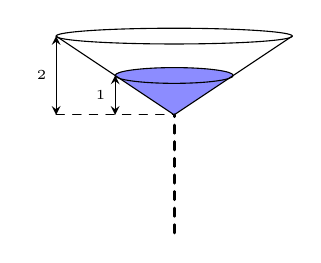
\begin{tikzpicture}[line cap=round,line join=round,>=stealth,x=1.0cm,y=1.0cm,scale=1]	
		\draw[fill=blue!45,line width = 0pt,draw=none](1.5,2)--(0.75,2.5)--(2.25,2.5);
		\draw[dashed,thin,line width=1pt] (1.5,0.5)--(1.5,2);
		\draw(3,3) arc (0:360:1.5 cm and 0.1 cm);
		\draw[fill=blue!45] (2.25,2.5) arc (0:360:0.75 cm and 0.1 cm);
		\draw (1.5,2)--(0,3);	
		\draw (1.5,2)--(3,3);
		\draw[<->] (0.75,2)--(0.75,2.5);
		\draw (0.75,2.25) node[left]{\tiny $1$};	
		\draw[<->] (0,2)--(0,3);
		\draw (0,2.5) node[left]{\tiny $2$};
		\draw [dashed] (0,2)--(1.5,2);
		\end{tikzpicture} ~~~~~~
		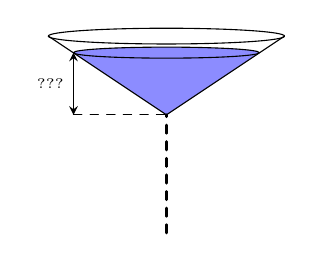
\begin{tikzpicture}[line cap=round,line join=round,>=stealth,x=1.0cm,y=1.0cm,scale=1]
		\draw[fill=blue!45,line width = 0pt,draw=none](1.5,2)--(0.32,2.79)--(2.68,2.79);
		\draw[dashed,thin,line width=1pt] (1.5,0.5)--(1.5,2);
		\draw(3,3) arc (0:360:1.5 cm and 0.1 cm);
		\draw[fill=blue!45] (2.68,2.79) arc (0:360:1.18 cm and 0.07 cm);
		\draw (1.5,2)--(0,3);
		\draw (1.5,2)--(3,3);
		\draw[<->] (0.32,2)--(0.32,2.79);
		\draw (0.32,2.39) node[left]{\tiny $???$};		
		\draw [dashed] (0.32,2)--(1.5,2);
		\end{tikzpicture} 
	\end{center}
	\choice
	{$h\approx 1,73 dm$}
	{$h\approx 1,89 dm$}
	{\True $h\approx 1,91 dm$}
	{$h\approx 1,41 dm$}
	\loigiai{
		\begin{center}
			\begin{tikzpicture}[scale=0.8,>=stealth, font=\footnotesize, line join=round, line cap=round]
		\tkzDefPoints{0/0/H,0/5/A,-3/0/B,3/0/C}
		\coordinate (D) at ($(A)!1/2!(H)$);
		\coordinate (M) at ($(A)!1/2!(B)$);
		\coordinate (N) at ($(A)!1/2!(C)$);
		\coordinate (F) at ($(A)!3/5!(H)$);
		\coordinate (E) at ($(A)!3/5!(B)$);
		\coordinate (I) at ($(A)!3/5!(C)$);
		\tkzDrawSegments(A,B B,C A,C A,H M,N E,I)
		\tkzDrawPoints[fill=black,size=5](A,B,C,D,F,H)
		\tkzLabelPoints[below](B,C,H)
		\tkzLabelPoints[above](A)
		\tkzLabelPoints[below right](F)
		\tkzLabelPoints[above right](D)
		\end{tikzpicture}
		\end{center}
		Có chiều cao hình nón khi đựng đầy nước ở ly thứ nhất: $AH=2$.\\
		Chiều cao phần nước ở ly thứ nhất sau khi đổ sang ly thứ hai: $AD=1$.\\
		Chiều cao phần nước ở ly thứ hai sau khi đổ sang ly thứ hai: $AF=h$.\\
		Theo Ta let ta có: $\dfrac{R'}{R}=\dfrac{AD}{AH}=\dfrac{1}{2}$, $\dfrac{R'}{R}=\dfrac{AF}{AH}=\dfrac{h}{2}$ suy ra $R'=\dfrac{R}{2}$, $R''=\dfrac{Rh}{2}$.\\
		Thể tích phần nước ban đầu ở ly thứ nhất: $V=2\pi R^2$.\\
		Thể tích phần nước ở ly thứ hai: $V_1=\pi R''^2h =\dfrac{\pi R^2h^3}{4}$.\\
		Thể tích phần nước còn lại ở ly thứ nhất: $V_2=\dfrac{\pi R^2}{4}$.\\
		Mà: $V=V_1+V_2\Leftrightarrow\dfrac{\pi R^2h^3}{4}+\dfrac{\pi R^2}{4}=2\pi R^2\Leftrightarrow\dfrac{h^3}{4}+\dfrac{1}{4}=2\Leftrightarrow h=\sqrt[3]{7}\approx 1,91$.}
\end{ex}
\begin{ex}%[2H2G1-5]%Câu 47.
	Một công ty sản xuất một loại cốc giấy hình nón có thể tích $27 cm^3$, với chiều cao $h$ và bán kính đáy $r$. Giá trị $r$ để lượng giấy tiêu thụ ít nhất: 
	\choice
	{$r=\sqrt[4]{\dfrac{3^6}{2{\pi}^2}}$}
	{\True $r=\sqrt[6]{\dfrac{3^8}{2{\pi}^2}}$}
	{$r=\sqrt[4]{\dfrac{3^8}{2{\pi}^2}}$}
	{$r=\sqrt[6]{\dfrac{3^6}{2{\pi}^2}}$}
	\loigiai{
		Ta có thể tích cốc hình nón $V=\dfrac{1}{3}\pi\cdot r^2\cdot h=27\Rightarrow h=\dfrac{81}{\pi\cdot r^2}$, $r>0$.\\
		Khi đó $l=\sqrt{\left(\dfrac{81}{\pi\cdot r^2}\right)^2+r^2}$. Suy ra:\\
		$S_{xq}=\pi\cdot r\cdot\sqrt{\left(\dfrac{81}{\pi\cdot r^2}\right)^2+r^2} =\pi\sqrt{r^2\left(\dfrac{3^8}{{\pi}^2\cdot r^4}+r^2\right)}=\pi\sqrt{\dfrac{3^8}{{\pi}^2\cdot r^2}+r^4}=\pi\sqrt{f(r)}$.\\
		Lượng giấy tiêu thụ ít nhất $\Leftrightarrow$ diện tích xung quanh phải nhỏ nhất $\Leftrightarrow f(r)$ nhỏ nhất.\\
		Ta có: $f(r)=\dfrac{3^8}{{\pi}^2\cdot r^2}+r^4=\dfrac{3^8}{2{\pi}^2\cdot r^2}+\dfrac{3^8}{2{\pi}^2\cdot r^2}+r^4\geq 3\sqrt[3]{\dfrac{(3^8)^2}{4{\pi}^4}}$.\\
		Đẳng thức xảy ra khi và chỉ khi $\dfrac{3^8}{2{\pi}^2\cdot r^2}=r^4\Leftrightarrow r^6=\dfrac{3^8}{2{\pi}^2}\Leftrightarrow r=\sqrt[6]{\dfrac{3^8}{2{\pi}^2}}$.\\
		Vậy để lượng giấy tiêu thụ ít nhất thì $r=\sqrt[6]{\dfrac{3^8}{2{\pi}^2}}$.\\
		Chú ý: Ta có thể khảo sát hàm $f(r)=\dfrac{3^8}{{\pi}^2\cdot r^2}+r^4$, $r>0$.\\
		$f'(r)=0\Leftrightarrow r=\sqrt[6]{\dfrac{3^8}{2{\pi}^2}}=r_0$. 
		\begin{center}
			
\begin{tikzpicture}
			\tkzTabInit[nocadre=false,lgt=1.2,espcl=2.5,deltacl=0.6]
			{$x$ /0.6,$f'$ /0.6,$f(r)$ /2}
			{$-\infty$,$r_o$,$+\infty$}
			\tkzTabLine{,-,$0$,+,}
			\tkzTabVar{+/$+\infty$, -/$f(r_o)$,+/$+\infty$}
			\end{tikzpicture}
		\end{center}}
\end{ex}
\begin{ex}%[2H2G2-4]%Câu 48.
	Có $4$ viên bi hình cầu có bán kính bằng $1$ cm. Người ta đặt $3$ viên bi tiếp xúc nhau và cùng tiếp xúc với mặt bàn. Sau đó đai chặt $3$ viên bi đó lại và đặt $1$ viên bi thứ $4$ tiếp xúc với cả $3$ viên bi trên như hình vẽ dưới đây
	\begin{center}
		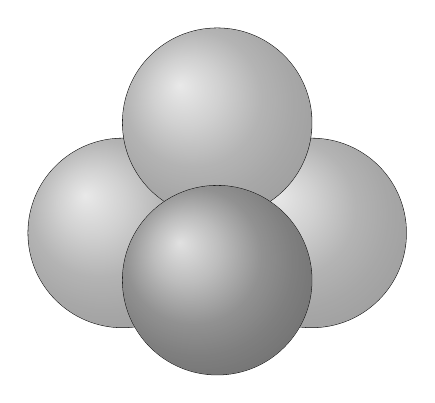
\begin{tikzpicture}[scale=0.6]
	%1
	\draw (2,1) circle (2cm);
	\fill[black!10]                (2,1) circle (2cm);
	\shade[ball color = gray!80, opacity = 0.4] (2,1) circle (2cm);
	%2
	\draw (-2,1) circle (2cm);
	\fill[black!10,  opaque] (-2,1) circle (2cm);
	\shade[ball color = gray!80, opacity = 0.4] (-2,1) circle (2cm);
	%4
	\draw (0,10/3) circle (2cm);
	\fill[black!10] (0,10/3) circle (2cm);
	\shade[ball color = gray!80, opacity = 0.4] (0,10/3) circle (2cm);
	%3
	\draw (0,0) circle (2cm);
	\fill[black!20] (0,0) circle (2cm);
	\shade[ball color = gray!80, opacity = 0.6] (0,0) circle (2cm);
	\tkzDefPoint(2,1){A}
	\tkzDefPoint(-2,1){B}
	\tkzDefPoint(0,0){C}
	\tkzDefPoint(0,2/3){D}
	\tkzDefPoint(0,10/3){E}
	\tkzDefPoint(0,1.4){I}
	\end{tikzpicture}
	\end{center}
	Gọi $O$ là điểm thuộc bề mặt của viên bi thứ tư có khoảng cách đến mặt bàn là lớn nhất. Khoảng cách từ $O$ đến mặt bàn bằng
	\choice
	{\True $\dfrac{6+2\sqrt{6}}{3}$}
	{$\dfrac{7}{2}$}
	{$\dfrac{3+2\sqrt{6}}{3}$}
	{$\dfrac{4\sqrt{6}}{3}$}
	\loigiai{
		\begin{center}
			\begin{tikzpicture}[scale=1,>=stealth, font=\footnotesize, line join=round, line cap=round]
		\tkzDefPoints{-2/0/I,2/0/J,0/0/H,-2/1/M,2/1/N,-1/1/A,0/1/K,1/1/C,0/2.733/L,0/3.733/O}
		\tkzDrawSegments(I,J)
		\tkzDrawSegments[dashed](M,N O,H)
		\tkzDrawPoints[fill=black,size=5](A,K,C,L,O,H)
		\draw (A) circle(1cm);
		\draw (C) circle(1cm);
		\draw (L) circle(1cm);
		\draw (K) circle(1cm);
		\tkzLabelPoints[below](A,C,H)
		\tkzLabelPoints[below right](K,L)
		\tkzLabelPoints[above](O)
		\end{tikzpicture}
		\begin{tikzpicture}[scale=0.8,>=stealth, font=\footnotesize, line join=round, line cap=round]
		\tkzDefPoints{0/0/A,1.2/-1.6/B,4.5/0/C}
		\tkzCentroid(A,B,C)\tkzGetPoint{K}
		\coordinate (L) at ($(K)+(0,3.5)$);
		\coordinate (M) at ($(B)!1/2!(C)$);
		\tkzDrawPolygon(A,B,C,L)
		\tkzDrawSegments(L,B L,A L,C A,B B,C)
		\tkzDrawSegments[dashed](M,A A,C L,K)
		\tkzDrawPoints[fill=black,size=4](A,B,C,L,K,M)
		\tkzMarkRightAngles[size=0.14](A,M,B L,K,A)
		\tkzLabelPoints[above](L)
		\tkzLabelPoints[below](B,K,M)
		\tkzLabelPoints[left](A)
		\tkzLabelPoints[right](C)
		\end{tikzpicture}
		\end{center}
		Nhận xét: Tâm $A$, tâm $B$, tâm $C$, tâm $L$ của bốn mặt cầu lập thành $1$ tứ diện đều cạnh bằng\\
		$2$ cm. Tức là, tứ diện $LABC$ đều cạnh bằng $2$ cm.\\
		Trong tam giác đều $ABC$, có $KC=\dfrac{2}{3}\cdot\dfrac{2\sqrt{3}}{2}=\dfrac{2\sqrt{3}}{3}$.\\
		Trong tam giác vuông $LKC$, có $LK=\sqrt{LC^2-KC^2}=\sqrt{2^2-\left(\dfrac{2\sqrt{3}}{3}\right)^2}=\dfrac{2\sqrt{6}}{3}$.\\		Khoảng cách từ $O$ đến mặt bàn bằng $d$, với $d=OL+LK+KH=1+\dfrac{2\sqrt{6}}{3}+1=\dfrac{6+2\sqrt{6}}{3}$.}
\end{ex}
\begin{ex}%[2H2G2-6]%Câu 49.
	Cho hình nón $(N)$ có góc ở đỉnh bằng $60^{\circ},$ độ dài đường sinh bằng $a$. Dãy hình cầu.\\
	$(S_1), (S_2), (S_3),\ldots, (S_n),\ldots$ thỏa mãn: $(S_1)$ tiếp xúc với mặt đáy và các đường sinh của hình nón $(N); (S_2)$ tiếp xúc ngoài với $(S_1)$ và tiếp xúc với các đường sinh của hình nón $(N); (S_3)$ tiếp xúc ngoài với $(S_2)$ và tiếp xúc với các đường sinh của hình nón $(N)$. Tính tổng thể tích các khối cầu $(S_1), (S_2), (S_3),\ldots, (S_n),\ldots$ theo $a$. 
	\choice
	{\True $\dfrac{\pi a^3\sqrt{3}}{52}$}
	{$\dfrac{27\pi a^3\sqrt{3}}{52}$}
	{$\dfrac{\pi a^3\sqrt{3}}{48}$}
	{$\dfrac{9\pi a^3\sqrt{3}}{16}$}
	\loigiai{
		\begin{center}
			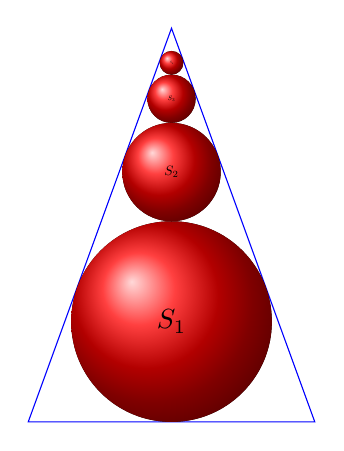
\begin{tikzpicture}
		\def\g{20}%Nửa góc ở đỉnh
		\def\h{5}%Chiều cao tam giác
		\def\n{3}%Số hình tròn
		\pgfmathsetmacro{\r}{\h *sin(\g)/(1+sin(\g))}
		\pgfmathsetmacro{\b}{\h-\r}
		\pgfmathsetmacro{\a}{\h *tan(\g)}
		\draw[blue] (90:\h)--(0:\a)--(180:\a)--cycle;
		\fill[ball color=red] (90:\r) circle (\r);
		\path (90:\h-\b) node{$S_{1}$};
		\foreach \i in {1,...,\n}{
			\pgfmathsetmacro{\j}{int(\i+1)}
			\pgfmathsetmacro{\tl}{((1-sin(\g))/(1+sin(\g)))^(\i)}
			\pgfmathsetmacro{\ri}{\r *\tl}
			\pgfmathsetmacro{\bi}{\b *\tl}
			\fill[ball color=red] (90:\h-\bi) circle (\ri);
			\path (90:\h-\bi) node[scale=\tl]{$S_{\j}$};
		}
		\end{tikzpicture}
		\begin{tikzpicture}
		\def\h{2}%đường cao lớn SH
		\pgfmathsetmacro{\a}{\h*sqrt(3)}
		\coordinate[label=below:$ H $] (H) at (0,0);
		\coordinate[label=below:$ B $] (B) at (-\a,0);
		\coordinate[label=below:$ A $] (A) at (\a,0);
		\coordinate[label=left:$ I_1 $] (I1) at (0,\h);
		\coordinate[label=below right:$ E $] (E) at ($ (I1)!-1!(H) $);
		\coordinate[label=left:$ I_2 $] (I2) at ($(E)!-1/3!(I1)$);
		\coordinate[label=above:$ S $] (S) at ($(I2)!-2!(E)$);
		\draw (I1) circle (\h) 
		(I2) circle (\h/3)
		(S)--(A)--(B)--(S)--(H);
		
		
		\fill[black](H) circle (1pt) 
		(I1) circle (1pt) 
		(I2) circle (1pt) 
		(E) circle (1pt);
		\end{tikzpicture}
		\end{center}
		Gọi $I_1,I_2$ lần lượt là tâm của mặt cầu $(S_1)$ và $(S_2)$.\\
		Gọi $H$ là trung điểm của $AB$. Khi đó ta có $\Delta SAB$ đều và $R_1=\dfrac{1}{3}SH=\dfrac{1}{3}\cdot\dfrac{a\sqrt{3}}{2}=\dfrac{a\sqrt{3}}{6}$.\\
		Hạ $I_1M_1\perp SA$, $I_2M_2\perp SA$.\\
		Xét $\Delta SI_2M_2$ có $\sin 30^{\circ}=\dfrac{I_2M_2}{SI_2}\Rightarrow SI_2=2I_2M_2$. Khi đó ta có $SH=SI_2+I_2E+EH$ \\
		$ \Leftrightarrow 3r_1=3r_2+2r_1\Leftrightarrow r_1=3r_2 $.\\
		Chứng minh tương tự ta có $r_2=3r_3$,…., $r_n=3r_{n+1}$.\\
		Do đó dãy bán kính $r_1$, $r_2$,…, $r_n$, lập thành một cấp số nhân lùi vô hạn với $r_1=\dfrac{a\sqrt{3}}{6}$ và công bội $q=\dfrac{1}{3}$.\\
		Suy ra dãy thể tích của các khối cầu $(S_1)$, $(S_2)$, …, $(S_n)$,… lập thành một cấp số nhân lùi vô hạn với $V_1=\dfrac{4}{3}\pi\cdot\left(\dfrac{a\sqrt{3}}{6}\right)^3=\dfrac{\sqrt{3}}{54}\pi a^3$ và công bội $q_1=\dfrac{1}{27}$.\\
		Vậy tổng thể tích của các khối cầu $(S_1),(S_2),\ldots,(S_n),\ldots$ là $V=\dfrac{V_1}{1-q}=\dfrac{\sqrt{3}}{52}\pi a^3$.}
\end{ex}
\begin{ex}%[2H2G2-6]%Câu 50.
	Cho mặt cầu $(S)$ bán kính $R$. Hình nón $(N)$ thay đổi có đỉnh và đường tròn đáy thuộc mặt cầu $(S)$. Thể tích lớn nhất của khối nón $(N)$ là 
	\choice
	{\True $\dfrac{32\pi R^3}{81}$}
	{$\dfrac{32R^3}{81}$}
	{$\dfrac{32\pi R^3}{27}$}
	{$\dfrac{32R^3}{27}$}
	\loigiai{
		\begin{center}
			\begin{tikzpicture}[scale=0.5,>=stealth, font=\footnotesize, line join=round, line cap=round]
		\tkzDefPoints{0/0/I,-4/0/A,0/3/O,0/8/S,4/0/B}
		\draw (O) circle(5cm);
		\tkzDrawSegments[dashed](A,I S,I A,O A,S B,S)
		\draw [dashed] (A) arc (180:0: 4cm and 1.0cm);
		\draw (A) arc (-180:0: 4cm and 1.0cm);
		\tkzLabelPoints[below](A,I)
		\tkzLabelPoints[above](S)
		\tkzLabelPoints[right](O)
		\end{tikzpicture}
		\end{center}
		Ta có thể tích khối nón đỉnh $S$ lớn hơn hoặc bằng thể tích khối nón đỉnh $S'$. Do đó chỉ cần xét khối nón đỉnh $S$ có bán kính đường tròn đáy là $r$ và đường cao là $SI=h$ với $h\geq R$.\\
		Thể tích khối nón được tạo nên bởi $(N)$ là\\
		$V=\dfrac{1}{3}h\cdot S_{(C)} =\dfrac{1}{3}h\cdot\pi\cdot r^2 =\dfrac{1}{3}h\cdot\pi\cdot\left[R^2-(h-R)^2\right] =\dfrac{1}{3}\pi\left(-h^3+2h^2R\right)$.\\
		Xét hàm số: $f(h)=-h^3+2h^2R$ với $h\in[R;2R)$.\\
		Ta có $f'(h)=-3h^2+4hR$.\\
		$f'(h)=0\Leftrightarrow-3h^2+4hR=0\Leftrightarrow h=0$ (loại) hoặc $h=\dfrac{4R}{3}$.\\
		Bảng biến thiên: 
		\begin{center}
			
\begin{tikzpicture}
			\tkzTabInit[nocadre=false,lgt=1.2,espcl=2.5,deltacl=0.6]
			{$h$ /0.8,$f'(h)$ /0.8,$f(h)$ /2}
			{$R$,$\frac{4R}{3}$,$2R$}
			\tkzTabLine{,+,$0$,-,}
			\tkzTabVar{-/$R^3$, +/$\dfrac{32R^3}{27}$,-/$0$}
			\end{tikzpicture}
		\end{center}
		Ta có: $\max f(h)=\dfrac{32}{27}R^3$ tại $h=\dfrac{4R}{3}$.\\
		Vậy thể tích khối nón được tạo nên bởi $(N)$ có giá trị lớn nhất là $V=\dfrac{1}{3}\pi\dfrac{32}{27}R^3=\dfrac{32}{81}\pi R^3$ khi $h=\dfrac{4R}{3}$.\\
		Chú ý: Sau khi tính được $V=\dfrac{1}{3}\pi\left(-h^3+2h^2R\right)$ ta có thể làm như sau:\\
		$V=\dfrac{1}{3}\pi\left(-h^3+2h^2R\right)=\dfrac{1}{3}\pi h^2(2R-h)=\dfrac{\pi}{6}\cdot h\cdot h(4R-2h)\leq\dfrac{\pi}{6}\left(\dfrac{h+h+4R-2h}{3}\right)^3=\dfrac{32\pi R^3}{81}$.\\
		Đẳng thức xảy ra khi và chỉ khi $h=4R-2h\Leftrightarrow h=\dfrac{4R}{3}$.}
\end{ex}
\Closesolutionfile{ans}
\DAPAN
\inputansbox{10}{ans/ansCD2H2-3OTC}
